% \usepackage{cite}
% \usepackage{amsmath,amssymb,amsfonts}
% \usepackage{algorithmic}
% \usepackage{graphicx}
% \usepackage{textcomp}
% \usepackage{xcolor}

% \usepackage{amsmath,amssymb,amsfonts}
% \usepackage{algorithmic}
% \usepackage{graphicx}
% \usepackage[inline, shortlabels]{enumitem}
% \usepackage{tabularx}
% \usepackage{caption}
% \usepackage{titlesec}
% \usepackage[T2A,T1]{fontenc}
% \usepackage[english]{babel}
% \captionsetup{font=it}
% \usepackage{ragged2e}
% \addto\extrasenglish{%
%   \renewcommand{\sectionautorefname}{Section}%
%   \renewcommand{\subsectionautorefname}{Subsection}%
%   \renewcommand{\subsubsectionautorefname}{Subsubsection}%
%   \renewcommand{\tableautorefname}{Table}%
%   \renewcommand{\figureautorefname}{Figure}%
% }
% \usepackage{pifont}
% \newcommand{\cmark}{\ding{51}}%
% \newcommand{\xmark}{\ding{55}}%
% \usepackage{footmisc}
% \usepackage{multirow}

% % --- Tickz
% \usepackage{physics}
% \usepackage{amsmath}
% \usepackage{tikz}
% \usepackage{mathdots}
% \usepackage{yhmath}
% \usepackage{float}
% \usepackage{pdfpages}
% \usepackage{stfloats}
% \usepackage{cancel}
% \usepackage{color}
% \usepackage{siunitx}
% \usepackage{array}
% \usepackage{multirow}
% \usepackage{amssymb}
% \usepackage{gensymb}
% \usepackage{tabularx}
% \usepackage{extarrows}
% \usepackage{booktabs}
% \usetikzlibrary{fadings}
% \usetikzlibrary{patterns}
% \usetikzlibrary{shadows.blur}
% \usetikzlibrary{shapes}

% % ---------

% \usepackage{pdfpages}
% \usepackage{booktabs}
% \usepackage{csquotes}
% \usepackage{lipsum}  
% \usepackage{arydshln}
% \usepackage{smartdiagram}
% \usepackage[inkscapeformat=png]{svg}
% \usepackage{textcomp}
% \usepackage{tabularray}\UseTblrLibrary{varwidth}
% \usepackage{xcolor}
% \def\BibTeX{{\rm B\kern-.05em{\sc i\kern-.025em b}\kern-.08em
%     T\kern-.1667em\lower.7ex\hbox{E}\kern-.125emX}}
% \usepackage{cite}
% \usepackage{amsmath}
% \newcommand{\probP}{\text{I\kern-0.15em P}}
% \usepackage{etoolbox}
% \patchcmd{\thebibliography}{\section*{\refname}}{}{}{}

% \usepackage{hyperref}
% \setlength{\extrarowheight}{2.5pt}

% % \renewcommand{\arraystretch}{1.7}

% % \setlength{\extrarowheight}{2.5pt}
% % \renewcommand{\arraystretch}{0.2}
% % \renewcommand{\arraystretch}{1.7}

% % --------------
% \titleclass{\subsubsubsection}{straight}[\subsection]

% \newcounter{subsubsubsection}[subsubsection]
% \renewcommand\thesubsubsubsection{\thesubsubsection.\arabic{subsubsubsection}}
% \renewcommand\theparagraph{\thesubsubsubsection.\arabic{paragraph}} % optional; useful if paragraphs are to be numbered

% \titleformat{\subsubsubsection}
%   {\normalfont\normalsize\bfseries}{\thesubsubsubsection}{1em}{}
% \titlespacing*{\subsubsubsection}
% {0pt}{3.25ex plus 1ex minus .2ex}{1.5ex plus .2ex}

% \makeatletter
% \renewcommand\paragraph{\@startsection{paragraph}{5}{\z@}%
%   {3.25ex \@plus1ex \@minus.2ex}%
%   {-1em}%
%   {\normalfont\normalsize\bfseries}}
% \renewcommand\subparagraph{\@startsection{subparagraph}{6}{\parindent}%
%   {3.25ex \@plus1ex \@minus .2ex}%
%   {-1em}%
%   {\normalfont\normalsize\bfseries}}
% \def\toclevel@subsubsubsection{4}
% \def\toclevel@paragraph{5}
% \def\toclevel@paragraph{6}
% \def\l@subsubsubsection{\@dottedtocline{4}{7em}{4em}}
% \def\l@paragraph{\@dottedtocline{5}{10em}{5em}}
% \def\l@subparagraph{\@dottedtocline{6}{14em}{6em}}
% \makeatother

% \makeatletter
% \newcommand{\linebreakand}{%
%   \end{@IEEEauthorhalign}
%   \hfill\mbox{}\par
%   \mbox{}\hfill\begin{@IEEEauthorhalign}
% }
% \makeatother

% \setcounter{secnumdepth}{4}
% \setcounter{tocdepth}{4}


% \setboolean{@twoside}{false}

% % --------------


% \newcommand{\before}[1]{\textcolor{red}{#1}}
% \newcommand{\after}[1]{\textcolor{green}{#1}}

% \newcommand{\old}[1]{\textcolor{orange}{#1}}
% \newcommand{\rem}[1]{\textcolor{red}{#1}}
% \newcommand{\todo}[1]{\textcolor{orange}{\newline \textit{\textbf{TODO:} #1}} \newline \newline }

% \def\BibTeX{{\rm B\kern-.05em{\sc i\kern-.025em b}\kern-.08em
%     T\kern-.1667em\lower.7ex\hbox{E}\kern-.125emX}}

\section{Introduction}
\label{sec:introduction}

% Contexte
Les systèmes critiques natifs du cloud dépendent de plus en plus de Kubernetes pour orchestrer et gérer des services interdépendants~\cite{Pahl2019}. HPA est un mécanisme largement adopté pour ajuster dynamiquement le nombre de pods en fonction de l'utilisation des ressources, permettant ainsi aux systèmes de gérer des charges de travail très dynamiques~\cite{Toka2020}. Cependant, des défaillances telles que les plantages de pods, les conflits de ressources et les goulots d'étranglement peuvent gravement compromettre les performances de toutes les fonctionnalités du cluster, que nous appelons globalement « résilience opérationnelle~\cite{burns2016borg}». Pire encore, ces défaillances peuvent être exploitées par des attaquants pour dégrader les performances ou provoquer des pannes, comme on le voit dans des contextes hostiles tels que les attaques DDoS~\cite{David2021}.

Bien que les attaques DDoS puissent sembler improbables dans des clusters d'entreprise isolés, de nombreuses organisations exposent leurs services via des passerelles d'entrée, ce qui en fait des cibles viables. En interne, des surcharges de type DDoS peuvent également résulter de configurations incorrectes, de dispositifs compromis ou d'exercices de red teaming. La prise en compte de tels scénarios adversaires s'inscrit dans les meilleures pratiques en matière de cybersécurité et contribue à garantir une auto-scaling robuste et tolérante aux pannes.

Dans de tels scénarios hostiles, des acteurs malveillants peuvent exploiter les mécanismes de mise à l'échelle, exposant ainsi les limites des systèmes HPA conventionnels. Les approches modernes ont cherché à combler ces lacunes en utilisant l'apprentissage par renforcement (RL), dans lequel un agent optimise un objectif global unique, tel que la minimisation de la latence ou de l'utilisation des ressources~\cite{Gari2021}. Si ces méthodes démontrent leur adaptabilité, elles s'avèrent souvent insuffisantes pour gérer divers scénarios de défaillance afin de maintenir la \textit{qualité de service} (QoS)~\cite{Liu2024}. Par exemple, il peut être beaucoup plus critique de donner la priorité aux réponses aux pannes en cascade des pods lors d'une attaque que de réduire la latence. Ces défis soulignent la nécessité d'un système d'auto-scaling capable d'équilibrer dynamiquement plusieurs sous-objectifs afin de maintenir toute la QoS et de maximiser la résilience opérationnelle.

Passer d'une optimisation à objectif unique à une approche multi-objectifs est complexe~\cite{Shoham2009MAS}. Dans des scénarios réels, la résilience opérationnelle ne peut se réduire à un seul objectif : l'optimisation de la latence peut entrer en conflit avec la garantie d'une haute disponibilité ou la limitation du surprovisionnement des ressources. Dans des conditions difficiles, par exemple, la priorité accordée à l'atténuation des attaques DDoS peut nécessiter de sacrifier la latence, tandis que la récupération après un crash de pod exige une réaffectation rapide des ressources. Un agent RL unique a du mal à répondre à ces priorités en raison de la difficulté à coordonner les réponses à des défaillances diverses~\cite{Jennings1998}.

En revanche, les MAS offrent un paradigme prometteur en décomposant l'objectif global de maximisation de la résilience opérationnelle en sous-objectifs gérés par des agents spécialisés~\cite{Shoham2009MAS}. Chaque agent se concentre sur un mode de défaillance ou un objectif de performance spécifique, ce qui facilite la spécialisation, améliore la coordination et permet un apprentissage évolutif des politiques dans le cadre de charges de travail dynamiques.

Dans un scénario antagoniste, chaque défenseur peut contribuer de manière collaborative à des actions d'échelle complémentaires afin d'atteindre son propre sous-objectif, ce qui permet des réponses plus résilientes et mieux adaptées au contexte face à un attaquant~\cite{Jennings1998}. Nous appelons l'ensemble de ces collaborations un HPA MAS. Un HPA MAS s'appuie en fait sur le cadre de cyberdéfense des agents autonomes intelligents de cybersécurité (AICA), qui peuvent être considérés comme des agents ayant des rôles et des missions spécialisés qui défendent en collaboration les systèmes contre les attaquants~\cite{Kott2018}.

% Problématique
Cependant, la conception de HPA MAS adaptés à un cluster présente des défis importants, tels que la nécessité d'une connaissance approfondie du cluster, la nature fastidieuse des processus de conception manuelle et la difficulté de garantir un comportement optimal des agents. De plus, les changements de cluster nécessitent de répéter le processus de conception, ce qui augmente les coûts opérationnels et la complexité.

% Contribution
Parmi les travaux méthodologiques, nous nous sommes inspirés de l'approche \textit{Assisted MAS Organization Engineering Approach} (AOMEA)~\cite{soule2024aomea}, qui semble la mieux adaptée aux défis de l'automatisation et de la sécurité. Sur la base de l'AOMEA, nous proposons le \textit{Kubernetes Autoscaling with Resilient Multi-Agent system} (KARMA) pour automatiser le processus de conception et de mise en œuvre à travers quatre phases séquentielles :
\begin{enumerate*}[label=\textbf{\arabic*)}, itemjoin={;\quad }]
    \item \textbf{Modélisation} : création d'un jumeau numérique du cluster à partir de traces réelles afin de simuler des scénarios de défaillance
    \item \textbf{Formation} : formation des agents dans le cadre d'une simulation à l'aide de rôles et de missions qui intègrent des stratégies explicites basées sur des règles et des directives
    \item \textbf{Analyse} : validation des comportements des agents formés et extraction d'informations sur la conception grâce à une analyse empirique
    \item \textbf{Transfert} : exécution des agents formés pour appliquer les comportements appris via l'API Kubernetes réelle.
\end{enumerate*}

Ce cadre permet de mettre à jour de manière itérative le modèle de simulation avec les nouvelles traces collectées, ce qui permet de s'adapter aux changements du cluster. Nous avons validé notre approche sur des scénarios adversaires issus de l'environnement Kubernetes « Chained Service ». Les MAS ont été générés avec une intervention manuelle minimale et font preuve d'originalité. Ils rivalisent avec les systèmes HPA de pointe, notamment AWARE~\cite{aware2023}, Gym-HPA~\cite{gymhpa2022} et Rlad-core~\cite{Rossi2019}, en termes de maximisation de la résilience opérationnelle.

% Organisation
Le reste est structuré comme suit :
\autoref{sec:related_work} passe en revue les techniques HPA existantes et leurs limites dans des environnements dynamiques.
\autoref{sec:proposed_approach} détaille notre cadre de travail en s'appuyant sur des concepts connexes pour chaque phase.
\autoref{sec:experiments} décrit le dispositif expérimental.
\autoref{sec:results} présente et discute les résultats.
\autoref{sec:conclusion} conclut et fournit des orientations pour l'avenir.

% ===================================

\section{Travaux connexes}
\label{sec:travaux_connexes}

\begin{table}[h!]
    \centering
    \caption{Aperçu KARMA concernant certains systèmes HPA}
    \label{tab:autoscaling_criteria}
    {\footnotesize
    \renewcommand{\arraystretch}{1.1}
    % \resizebox{0.5\textwidth}{!}{%
    \begin{tabular}{>{\raggedright\arraybackslash}m{1.3cm}>{\centering\arraybackslash}m{0.6cm}>{\centering\arraybackslash}m{0.6cm}>{\centering\arraybackslash}m{0.6cm}>{\centering\arraybackslash}m{0.6cm}>{\centering\arraybackslash}m{0.6cm}>{\centering\arraybackslash}m{0.6cm}>{\centering\arraybackslash}m{0,6cm}>{\centering\arraybackslash}m{0,6cm}>{\centering\arraybackslash}m{0,6cm}}
    \hline
    \textbf{Critère} & \vspace{-0.3cm}\textbf{\cite{gymhpa2022}} & \vspace{-0.3cm}\textbf{\cite{aware2023}} & \vspace{-0.3cm}\textbf{\cite{Rossi2019}} & \vspace{-0.3cm}\textbf{\cite{QoSRL}} & \vspace{-0.3cm}\textbf{\cite{Zhou2024}} & \vspace{-0.3cm}\textbf{\cite{KOSMOS}} & \vspace{-0.3cm}\textbf{\cite{COPA}} \\
    \hline
    \hline
    Scénarios adversaires & Non & Partiel & Non & Non & Non & Non & Partiel \\
    \hline
    Multi-objectifs & Non & Oui & Partiel & Oui & Non & Oui & Non \\
    \hline
    Automatisation & Élevé & Moyen & Moyen & Élevé & Moyen & Moyen & Moyen \\
    \hline
    Apprentissage & Oui & Oui & Oui & Oui & Non & Non & Non \\
    \hline
    MAS & Non & Non & Non & Non & Non & Non & Non \\
    \hline
    Simulation & Oui & Non & Oui & Oui & Non & Non & Non \\
    \hline
    Environnement réel & Non & Oui & Oui & Oui & Oui & Oui & Oui \\
    \hline
    Expliquable & Non & Non & Non & Non & Non & Non & Non \\
    \hline
    Adaptation & Élevée & Moyenne & Moyenne & Moyenne & Élevée & Élevée & Moyenne \\
    \hline
    Garanties de sécurité & Non & Non & Non & Non & Non & Non & Non \\
    \hline
    \end{tabular}%
    }
  \end{table}


\noindent L'autoscaling dans Kubernetes repose traditionnellement sur des approches basées sur des métriques, telles que le Kubernetes Horizontal Pod Autoscaler (KHPA) par défaut, qui ajuste le nombre de pods en fonction de l'utilisation du CPU et de la mémoire~\cite{Carrion2022}. Bien qu'efficaces pour la mise à l'échelle de base, ces méthodes ne permettent pas de gérer les charges de travail dynamiques ou adverses, car elles reposent sur des règles réactives basées sur des seuils~\cite{Tran2022}. Pour surmonter ces limites, les recherches récentes se sont tournées vers l'apprentissage automatique (ML) et le RL.

% \subsection*{Systèmes basés sur l'apprentissage par renforcement}
Trois systèmes basés sur le RL se distinguent par leurs approches innovantes, leur applicabilité et leur pertinence :
%
\begin{itemize}
    \item \textbf{Gym-HPA}~\cite{gymhpa2022} sert d'environnement de référence pour l'apprentissage par renforcement, permettant d'expérimenter divers algorithmes d'apprentissage par renforcement. Il excelle dans l'adaptabilité à des charges de travail simulées avec un haut degré d'automatisation, mais manque de prise en charge multi-objectifs, d'explicabilité et d'applicabilité dans le monde réel
    \item \textbf{AWARE}~\cite{aware2023} intègre l'apprentissage par renforcement pour optimiser les décisions d'auto-scaling tout en équilibrant les objectifs de qualité de service, tels que le temps de réponse et le débit. Il prend partiellement en compte les scénarios adversaires, mais rencontre des difficultés avec les niveaux d'automatisation élevés et la coordination multi-agents.
    \item \textbf{Rlad-core}~\cite{Rossi2019} se concentre à la fois sur la mise à l'échelle horizontale et verticale en introduisant un système auto-adaptatif qui ajuste dynamiquement l'allocation des ressources en fonction des variations de la charge de travail, optimisant ainsi les performances tout en minimisant les coûts.
\end{itemize}

Ces systèmes mettent en évidence des progrès significatifs dans le domaine de l'auto-scaling basé sur le RL, mais présentent des limites communes : un manque d'adaptabilité globale face à des scénarios adversaires, un soutien limité aux MAS et aucune attention particulière accordée à l'explicabilité ou aux garanties de sécurité.
%
% \subsection*{Approches hybrides et basées sur des règles}
D'autres systèmes notables combinent des stratégies basées sur le ML ou sur des règles avec l'autoscaling traditionnel :
%
\begin{enumerate*}[label={}, itemjoin={;\quad }]
    \item \textbf{QoS-Aware RL}~\cite{QoSRL} se concentre sur le maintien de la qualité de service (QoS) sous des charges de travail dynamiques, mais ne s'intègre pas de manière transparente aux fonctionnalités natives de Kubernetes et ne prend pas en compte les scénarios adversaires
    \item \textbf{AHPA}~\cite{Zhou2024} et \textbf{KOSMOS}~\cite{KOSMOS} explorent des stratégies de mise à l'échelle verticale et horizontale adaptatives et combinées, offrant une grande adaptabilité mais manquant de capacités d'apprentissage
    \item \textbf{COPA}~\cite{COPA} met l'accent sur l'auto-scaling combiné basé sur des métriques, mais reste réactif et limité dans les scénarios adversaires.
\end{enumerate*}

% \subsection*{Positionnement de notre contribution}
KARMA comble les lacunes clés en matière de \textbf{(1) résilience opérationnelle} pour l'auto-scaling en introduisant un cadre de conception HPA MAS automatisé. Contrairement aux approches conventionnelles, qui échouent souvent dans des \textbf{(2) conditions adverses}, KARMA décompose le maintien de la résilience opérationnelle en missions et rôles spécifiques aux défaillances, permettant aux agents de gérer une réponse coordonnée aux \textbf{goulots d'étranglement}, aux \textbf{conflits de ressources}, aux \textbf{attaques DDoS} et aux \textbf{plages de pods}. Il combine \textbf{(3) la modélisation de jumeaux numériques} avec \textbf{(4) la génération automatisée de MAS} via l'apprentissage par renforcement multi-agents (MARL) intégrant la \textbf{satisfaction des contraintes} à ces rôles et missions, rationalisant ainsi la conception de HPA MAS avec un minimum d'intervention manuelle. Tirant parti de cette décomposition, KARMA recherche une meilleure \textbf{(5) adaptabilité} tout en permettant une meilleure \textbf{(6) explicabilité} de la prise de décision dans l'ensemble du HPA MAS.


% ===================================
\section{KARMA : un cadre pour la conception et le développement de HPA MAS}
\label{sec:approche_proposée}

\label{sec:approche_proposée}

Cette section présente le cadre KARMA qui aide à concevoir un HPA MAS, puis détaille chacune de ses phases.

\subsection{Présentation de KARMA}

\begin{figure}[h!]
    \centering
    


\tikzset{every picture/.style={line width=0.75pt}} %set default line width to 0.75pt        

\begin{tikzpicture}[x=0.75pt,y=0.75pt,yscale=-1.2,xscale=1.2]
%uncomment if require: \path (0,1414); %set diagram left start at 0, and has height of 1414

%Straight Lines [id:da5609883377896374] 
\draw [color={rgb, 255:red, 74; green, 144; blue, 226 }  ,draw opacity=1 ][line width=2.25]    (317.22,111.13) -- (360.07,111.13) ;
\draw [shift={(365.07,111.13)}, rotate = 180] [fill={rgb, 255:red, 74; green, 144; blue, 226 }  ,fill opacity=1 ][line width=0.08]  [draw opacity=0] (5.72,-2.75) -- (0,0) -- (5.72,2.75) -- cycle    ;
%Image [id:dp9396292457736715] 
\draw (106.77,60.95) node  {
\includegraphics[width=18.66pt,height=18.36pt]{figures/karma_architecture/pod.png}};
%Image [id:dp3874378335758297] 
\draw (145.86,60.95) node  {
\includegraphics[width=18.66pt,height=18.36pt]{figures/karma_architecture/pod.png}};
%Shape: Rectangle [id:dp4562827234223257] 
\draw  [color={rgb, 255:red, 74; green, 144; blue, 226 }  ,draw opacity=1 ][line width=1.5]  (89,28.36) .. controls (89,25.6) and (91.24,23.36) .. (94,23.36) -- (255,23.36) .. controls (257.76,23.36) and (260,25.6) .. (260,28.36) -- (260,132) .. controls (260,134.76) and (257.76,137) .. (255,137) -- (94,137) .. controls (91.24,137) and (89,134.76) .. (89,132) -- cycle ;
%Image [id:dp9455935833751838] 
\draw (172.5,16.24) node  {
\includegraphics[width=18.66pt,height=18.36pt]{figures/karma_architecture/kubernetes.png}};
%Shape: Rectangle [id:dp9564725691593288] 
\draw  [color={rgb, 255:red, 74; green, 144; blue, 226 }  ,draw opacity=1 ][line width=1.5]  (92.55,50.21) .. controls (92.55,47.45) and (94.79,45.21) .. (97.55,45.21) -- (155.08,45.21) .. controls (157.84,45.21) and (160.08,47.45) .. (160.08,50.21) -- (160.08,70.81) .. controls (160.08,73.57) and (157.84,75.81) .. (155.08,75.81) -- (97.55,75.81) .. controls (94.79,75.81) and (92.55,73.57) .. (92.55,70.81) -- cycle ;
%Image [id:dp9120856447688912] 
\draw (126.32,39.97) node  {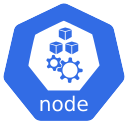
\includegraphics[width=18.66pt,height=18.36pt]{figures/karma_architecture/node.png}};
%Image [id:dp5738167237736518] 
\draw (106.77,119.52) node  {
\includegraphics[width=18.66pt,height=18.36pt]{figures/karma_architecture/pod.png}};
%Image [id:dp2199681121060142] 
\draw (145.86,119.52) node  {
\includegraphics[width=18.66pt,height=18.36pt]{figures/karma_architecture/pod.png}};
%Shape: Rectangle [id:dp12159705904547402] 
\draw  [color={rgb, 255:red, 74; green, 144; blue, 226 }  ,draw opacity=1 ][line width=1.5]  (92.55,108.78) .. controls (92.55,106.02) and (94.79,103.78) .. (97.55,103.78) -- (155.08,103.78) .. controls (157.84,103.78) and (160.08,106.02) .. (160.08,108.78) -- (160.08,129.38) .. controls (160.08,132.14) and (157.84,134.38) .. (155.08,134.38) -- (97.55,134.38) .. controls (94.79,134.38) and (92.55,132.14) .. (92.55,129.38) -- cycle ;
%Image [id:dp37768653229718074] 
\draw (126.32,98.54) node  {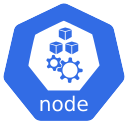
\includegraphics[width=18.66pt,height=18.36pt]{figures/karma_architecture/node.png}};
%Shape: Rectangle [id:dp20840815212238661] 
\draw  [color={rgb, 255:red, 74; green, 144; blue, 226 }  ,draw opacity=1 ][line width=1.5]  (264,28.36) .. controls (264,25.6) and (266.24,23.36) .. (269,23.36) -- (411.78,23.36) .. controls (414.54,23.36) and (416.78,25.6) .. (416.78,28.36) -- (416.78,132) .. controls (416.78,134.76) and (414.54,137) .. (411.78,137) -- (269,137) .. controls (266.24,137) and (264,134.76) .. (264,132) -- cycle ;
%Straight Lines [id:da9232180983272227] 
\draw [color={rgb, 255:red, 74; green, 144; blue, 226 }  ,draw opacity=1 ][line width=2.25]    (164,112) -- (201,112) ;
\draw [shift={(206,112)}, rotate = 180] [fill={rgb, 255:red, 74; green, 144; blue, 226 }  ,fill opacity=1 ][line width=0.08]  [draw opacity=0] (5.72,-2.75) -- (0,0) -- (5.72,2.75) -- cycle    ;
%Straight Lines [id:da6082715106712999] 
\draw [color={rgb, 255:red, 74; green, 144; blue, 226 }  ,draw opacity=1 ][line width=2.25]    (180,90.22) -- (167,90.22) ;
\draw [shift={(162,90.22)}, rotate = 360] [fill={rgb, 255:red, 74; green, 144; blue, 226 }  ,fill opacity=1 ][line width=0.08]  [draw opacity=0] (5.72,-2.75) -- (0,0) -- (5.72,2.75) -- cycle    ;
%Straight Lines [id:da30764510910060716] 
\draw [color={rgb, 255:red, 74; green, 144; blue, 226 }  ,draw opacity=1 ][line width=2.25]    (210,72) -- (199,72) ;
\draw [shift={(194,72)}, rotate = 360] [fill={rgb, 255:red, 74; green, 144; blue, 226 }  ,fill opacity=1 ][line width=0.08]  [draw opacity=0] (5.72,-2.75) -- (0,0) -- (5.72,2.75) -- cycle    ;
%Straight Lines [id:da5394403186779959] 
\draw [color={rgb, 255:red, 74; green, 144; blue, 226 }  ,draw opacity=1 ][line width=2.25]    (178,56.22) -- (167,56.22) ;
\draw [shift={(162,56.22)}, rotate = 360] [fill={rgb, 255:red, 74; green, 144; blue, 226 }  ,fill opacity=1 ][line width=0.08]  [draw opacity=0] (5.72,-2.75) -- (0,0) -- (5.72,2.75) -- cycle    ;
%Straight Lines [id:da6399475815904785] 
\draw [color={rgb, 255:red, 74; green, 144; blue, 226 }  ,draw opacity=1 ][line width=2.25]    (272,72) -- (235,72) ;
\draw [shift={(230,72)}, rotate = 360] [fill={rgb, 255:red, 74; green, 144; blue, 226 }  ,fill opacity=1 ][line width=0.08]  [draw opacity=0] (5.72,-2.75) -- (0,0) -- (5.72,2.75) -- cycle    ;
%Straight Lines [id:da24320102833940327] 
\draw [color={rgb, 255:red, 74; green, 144; blue, 226 }  ,draw opacity=1 ][line width=2.25]    (267,112) -- (230,112) ;
\draw [shift={(272,112)}, rotate = 180] [fill={rgb, 255:red, 74; green, 144; blue, 226 }  ,fill opacity=1 ][line width=0.08]  [draw opacity=0] (5.72,-2.75) -- (0,0) -- (5.72,2.75) -- cycle    ;
%Shape: Rectangle [id:dp9149123987409296] 
\draw  [color={rgb, 255:red, 255; green, 255; blue, 255 }  ,draw opacity=1 ][fill={rgb, 255:red, 255; green, 255; blue, 255 }  ,fill opacity=1 ] (328.83,106.67) -- (353.11,106.67) -- (353.11,114) -- (328.83,114) -- cycle ;
%Image [id:dp7127891043436136] 
\draw (341.68,109.47) node  {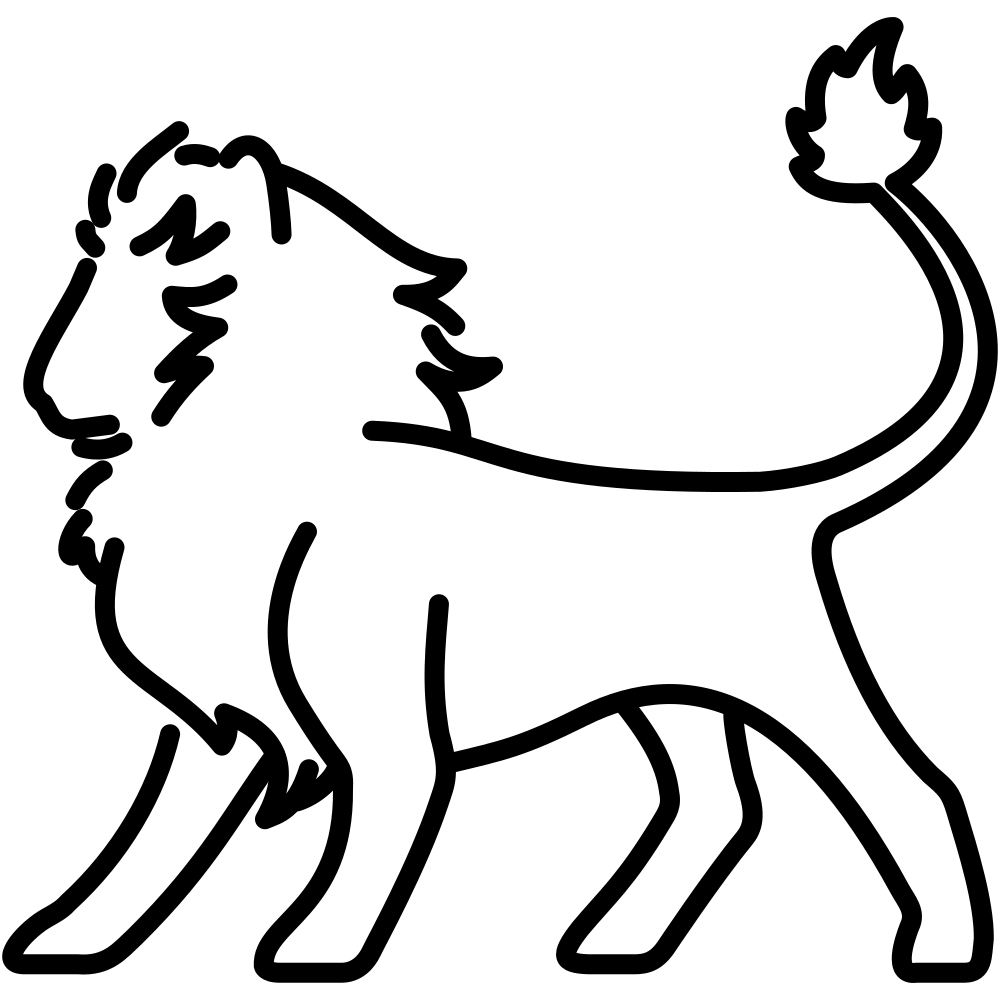
\includegraphics[width=14.57pt,height=15.21pt]{figures/karma_architecture/pettingzoo.png}};
%Straight Lines [id:da5757027637146572] 
\draw [color={rgb, 255:red, 74; green, 144; blue, 226 }  ,draw opacity=1 ][line width=2.25]    (357.9,41) -- (364.9,41) ;
\draw [shift={(352.9,41)}, rotate = 0] [fill={rgb, 255:red, 74; green, 144; blue, 226 }  ,fill opacity=1 ][line width=0.08]  [draw opacity=0] (5.72,-2.75) -- (0,0) -- (5.72,2.75) -- cycle    ;
%Straight Lines [id:da29364722138505184] 
\draw [color={rgb, 255:red, 74; green, 144; blue, 226 }  ,draw opacity=1 ][line width=2.25]    (390.99,97.77) -- (390.99,57.25) ;
\draw [shift={(390.99,52.25)}, rotate = 90] [fill={rgb, 255:red, 74; green, 144; blue, 226 }  ,fill opacity=1 ][line width=0.08]  [draw opacity=0] (5.72,-2.75) -- (0,0) -- (5.72,2.75) -- cycle    ;
%Straight Lines [id:da5470457469462804] 
\draw [color={rgb, 255:red, 74; green, 144; blue, 226 }  ,draw opacity=1 ][line width=2.25]    (390.9,71) -- (325.9,71) ;
\draw [shift={(320.9,71)}, rotate = 360] [fill={rgb, 255:red, 74; green, 144; blue, 226 }  ,fill opacity=1 ][line width=0.08]  [draw opacity=0] (5.72,-2.75) -- (0,0) -- (5.72,2.75) -- cycle    ;
%Shape: Rectangle [id:dp8476965567779329] 
\draw  [color={rgb, 255:red, 255; green, 255; blue, 255 }  ,draw opacity=1 ][fill={rgb, 255:red, 255; green, 255; blue, 255 }  ,fill opacity=1 ] (378.41,65.11) -- (397.83,65.11) -- (397.83,92) -- (378.41,92) -- cycle ;
%Shape: Smiley Face [id:dp8656850497140396] 
\draw  [fill={rgb, 255:red, 255; green, 255; blue, 255 }  ,fill opacity=1 ][line width=0.75]  (380.35,69.4) .. controls (380.35,67.3) and (382.09,65.6) .. (384.24,65.6) .. controls (386.38,65.6) and (388.12,67.3) .. (388.12,69.4) .. controls (388.12,71.5) and (386.38,73.2) .. (384.24,73.2) .. controls (382.09,73.2) and (380.35,71.5) .. (380.35,69.4) -- cycle ; \draw  [fill={rgb, 255:red, 255; green, 255; blue, 255 }  ,fill opacity=1 ][line width=0.75]  (382.53,68.11) .. controls (382.53,67.9) and (382.7,67.73) .. (382.92,67.73) .. controls (383.13,67.73) and (383.31,67.9) .. (383.31,68.11) .. controls (383.31,68.32) and (383.13,68.49) .. (382.92,68.49) .. controls (382.7,68.49) and (382.53,68.32) .. (382.53,68.11) -- cycle ; \draw  [fill={rgb, 255:red, 255; green, 255; blue, 255 }  ,fill opacity=1 ][line width=0.75]  (385.17,68.11) .. controls (385.17,67.9) and (385.34,67.73) .. (385.56,67.73) .. controls (385.77,67.73) and (385.95,67.9) .. (385.95,68.11) .. controls (385.95,68.32) and (385.77,68.49) .. (385.56,68.49) .. controls (385.34,68.49) and (385.17,68.32) .. (385.17,68.11) -- cycle ; \draw  [line width=0.75]  (382.29,70.92) .. controls (383.59,71.94) and (384.88,71.94) .. (386.18,70.92) ;
%Shape: Smiley Face [id:dp9163740789669144] 
\draw  [fill={rgb, 255:red, 255; green, 255; blue, 255 }  ,fill opacity=1 ][line width=0.75]  (392.01,69.4) .. controls (392.01,67.3) and (393.75,65.6) .. (395.89,65.6) .. controls (398.04,65.6) and (399.78,67.3) .. (399.78,69.4) .. controls (399.78,71.5) and (398.04,73.2) .. (395.89,73.2) .. controls (393.75,73.2) and (392.01,71.5) .. (392.01,69.4) -- cycle ; \draw  [fill={rgb, 255:red, 255; green, 255; blue, 255 }  ,fill opacity=1 ][line width=0.75]  (394.18,68.11) .. controls (394.18,67.9) and (394.36,67.73) .. (394.57,67.73) .. controls (394.79,67.73) and (394.96,67.9) .. (394.96,68.11) .. controls (394.96,68.32) and (394.79,68.49) .. (394.57,68.49) .. controls (394.36,68.49) and (394.18,68.32) .. (394.18,68.11) -- cycle ; \draw  [fill={rgb, 255:red, 255; green, 255; blue, 255 }  ,fill opacity=1 ][line width=0.75]  (396.82,68.11) .. controls (396.82,67.9) and (397,67.73) .. (397.21,67.73) .. controls (397.43,67.73) and (397.6,67.9) .. (397.6,68.11) .. controls (397.6,68.32) and (397.43,68.49) .. (397.21,68.49) .. controls (397,68.49) and (396.82,68.32) .. (396.82,68.11) -- cycle ; \draw  [line width=0.75]  (393.95,70.92) .. controls (395.24,71.94) and (396.54,71.94) .. (397.83,70.92) ;
%Shape: Smiley Face [id:dp8186451078369623] 
\draw  [fill={rgb, 255:red, 255; green, 255; blue, 255 }  ,fill opacity=1 ][line width=0.75]  (386.18,77.44) .. controls (386.18,75.34) and (387.92,73.64) .. (390.06,73.64) .. controls (392.21,73.64) and (393.95,75.34) .. (393.95,77.44) .. controls (393.95,79.54) and (392.21,81.24) .. (390.06,81.24) .. controls (387.92,81.24) and (386.18,79.54) .. (386.18,77.44) -- cycle ; \draw  [fill={rgb, 255:red, 255; green, 255; blue, 255 }  ,fill opacity=1 ][line width=0.75]  (388.36,76.15) .. controls (388.36,75.94) and (388.53,75.77) .. (388.74,75.77) .. controls (388.96,75.77) and (389.13,75.94) .. (389.13,76.15) .. controls (389.13,76.36) and (388.96,76.53) .. (388.74,76.53) .. controls (388.53,76.53) and (388.36,76.36) .. (388.36,76.15) -- cycle ; \draw  [fill={rgb, 255:red, 255; green, 255; blue, 255 }  ,fill opacity=1 ][line width=0.75]  (391,76.15) .. controls (391,75.94) and (391.17,75.77) .. (391.39,75.77) .. controls (391.6,75.77) and (391.77,75.94) .. (391.77,76.15) .. controls (391.77,76.36) and (391.6,76.53) .. (391.39,76.53) .. controls (391.17,76.53) and (391,76.36) .. (391,76.15) -- cycle ; \draw  [line width=0.75]  (388.12,78.96) .. controls (389.42,79.98) and (390.71,79.98) .. (392.01,78.96) ;
%Flowchart: Punched Tape [id:dp6020643269389074] 
\draw  [fill={rgb, 255:red, 255; green, 255; blue, 255 }  ,fill opacity=1 ] (313.9,33.81) .. controls (313.9,35.03) and (318.18,36.02) .. (323.45,36.02) .. controls (328.73,36.02) and (333,35.03) .. (333,33.81) .. controls (333,32.58) and (337.28,31.59) .. (342.55,31.59) .. controls (347.83,31.59) and (352.1,32.58) .. (352.1,33.81) -- (352.1,51.52) .. controls (352.1,50.3) and (347.83,49.31) .. (342.55,49.31) .. controls (337.28,49.31) and (333,50.3) .. (333,51.52) .. controls (333,52.75) and (328.73,53.74) .. (323.45,53.74) .. controls (318.18,53.74) and (313.9,52.75) .. (313.9,51.52) -- cycle ;
%Straight Lines [id:da950307097731951] 
\draw [line width=0.75]    (324.14,41.04) -- (341.9,41) ;
%Shape: Smiley Face [id:dp8914579811118104] 
\draw  [line width=0.75]  (320.58,40.88) .. controls (320.58,39.7) and (321.59,38.73) .. (322.85,38.73) .. controls (324.1,38.73) and (325.11,39.7) .. (325.11,40.88) .. controls (325.11,42.07) and (324.1,43.03) .. (322.85,43.03) .. controls (321.59,43.03) and (320.58,42.07) .. (320.58,40.88) -- cycle ; \draw  [line width=0.75]  (321.85,40.15) .. controls (321.85,40.03) and (321.95,39.94) .. (322.08,39.94) .. controls (322.2,39.94) and (322.3,40.03) .. (322.3,40.15) .. controls (322.3,40.27) and (322.2,40.37) .. (322.08,40.37) .. controls (321.95,40.37) and (321.85,40.27) .. (321.85,40.15) -- cycle ; \draw  [line width=0.75]  (323.39,40.15) .. controls (323.39,40.03) and (323.49,39.94) .. (323.62,39.94) .. controls (323.74,39.94) and (323.84,40.03) .. (323.84,40.15) .. controls (323.84,40.27) and (323.74,40.37) .. (323.62,40.37) .. controls (323.49,40.37) and (323.39,40.27) .. (323.39,40.15) -- cycle ; \draw  [line width=0.75]  (321.71,41.74) .. controls (322.47,42.31) and (323.22,42.31) .. (323.98,41.74) ;
%Shape: Smiley Face [id:dp07941198495535606] 
\draw  [line width=0.75]  (329.9,45.15) .. controls (329.9,43.96) and (330.92,43) .. (332.17,43) .. controls (333.42,43) and (334.44,43.96) .. (334.44,45.15) .. controls (334.44,46.33) and (333.42,47.29) .. (332.17,47.29) .. controls (330.92,47.29) and (329.9,46.33) .. (329.9,45.15) -- cycle ; \draw  [line width=0.75]  (331.17,44.42) .. controls (331.17,44.3) and (331.28,44.2) .. (331.4,44.2) .. controls (331.53,44.2) and (331.63,44.3) .. (331.63,44.42) .. controls (331.63,44.54) and (331.53,44.63) .. (331.4,44.63) .. controls (331.28,44.63) and (331.17,44.54) .. (331.17,44.42) -- cycle ; \draw  [line width=0.75]  (332.72,44.42) .. controls (332.72,44.3) and (332.82,44.2) .. (332.94,44.2) .. controls (333.07,44.2) and (333.17,44.3) .. (333.17,44.42) .. controls (333.17,44.54) and (333.07,44.63) .. (332.94,44.63) .. controls (332.82,44.63) and (332.72,44.54) .. (332.72,44.42) -- cycle ; \draw  [line width=0.75]  (331.04,46.01) .. controls (331.79,46.58) and (332.55,46.58) .. (333.3,46.01) ;
%Shape: Smiley Face [id:dp8353415903298282] 
\draw  [line width=0.75]  (341.9,40.85) .. controls (341.9,39.67) and (342.92,38.71) .. (344.17,38.71) .. controls (345.42,38.71) and (346.44,39.67) .. (346.44,40.85) .. controls (346.44,42.04) and (345.42,43) .. (344.17,43) .. controls (342.92,43) and (341.9,42.04) .. (341.9,40.85) -- cycle ; \draw  [line width=0.75]  (343.17,40.12) .. controls (343.17,40) and (343.28,39.91) .. (343.4,39.91) .. controls (343.53,39.91) and (343.63,40) .. (343.63,40.12) .. controls (343.63,40.24) and (343.53,40.34) .. (343.4,40.34) .. controls (343.28,40.34) and (343.17,40.24) .. (343.17,40.12) -- cycle ; \draw  [line width=0.75]  (344.72,40.12) .. controls (344.72,40) and (344.82,39.91) .. (344.94,39.91) .. controls (345.07,39.91) and (345.17,40) .. (345.17,40.12) .. controls (345.17,40.24) and (345.07,40.34) .. (344.94,40.34) .. controls (344.82,40.34) and (344.72,40.24) .. (344.72,40.12) -- cycle ; \draw  [line width=0.75]  (343.04,41.71) .. controls (343.79,42.28) and (344.55,42.28) .. (345.3,41.71) ;
%Straight Lines [id:da21936285199788075] 
\draw [line width=0.75]    (324.19,41.87) -- (329.9,45) ;
%Image [id:dp05694376090002984] 
\draw (218.44,70.24) node  {
\includegraphics[width=18.66pt,height=18.36pt]{figures/karma_architecture/api.png}};
%Image [id:dp7747210194064744] 
\draw (186.74,54.54) node  {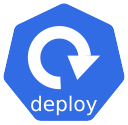
\includegraphics[width=18.66pt,height=18.36pt]{figures/karma_architecture/deploy.png}};
%Image [id:dp5268588430037433] 
\draw (186.74,87.76) node  {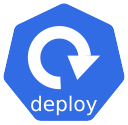
\includegraphics[width=18.66pt,height=18.36pt]{figures/karma_architecture/deploy.png}};
%Image [id:dp7447308292951857] 
\draw (218.44,111.76) node  {
\includegraphics[width=18.66pt,height=18.36pt]{figures/karma_architecture/prometheus.png}};
%Shape: Rectangle [id:dp7837974954754439] 
\draw  [color={rgb, 255:red, 75; green, 101; blue, 225 }  ,draw opacity=1 ][fill={rgb, 255:red, 74; green, 144; blue, 226 }  ,fill opacity=1 ] (202.37,94.64) -- (208.29,94.64) -- (208.29,101.67) -- (202.37,101.67) -- cycle ;
%Shape: Rectangle [id:dp780870970882084] 
\draw  [color={rgb, 255:red, 75; green, 101; blue, 225 }  ,draw opacity=1 ][fill={rgb, 255:red, 74; green, 144; blue, 226 }  ,fill opacity=1 ] (286.37,126) -- (292.29,126) -- (292.29,133.03) -- (286.37,133.03) -- cycle ;

%Shape: Rectangle [id:dp7051683429553395] 
\draw  [color={rgb, 255:red, 75; green, 101; blue, 225 }  ,draw opacity=1 ][fill={rgb, 255:red, 74; green, 144; blue, 226 }  ,fill opacity=1 ] (397.37,124.64) -- (403.29,124.64) -- (403.29,131.67) -- (397.37,131.67) -- cycle ;

%Shape: Rectangle [id:dp5578959475333973] 
\draw  [color={rgb, 255:red, 75; green, 101; blue, 225 }  ,draw opacity=1 ][fill={rgb, 255:red, 74; green, 144; blue, 226 }  ,fill opacity=1 ] (368.37,54.64) -- (374.29,54.64) -- (374.29,61.67) -- (368.37,61.67) -- cycle ;

%Shape: Rectangle [id:dp2822949836407178] 
\draw  [color={rgb, 255:red, 75; green, 101; blue, 225 }  ,draw opacity=1 ][fill={rgb, 255:red, 74; green, 144; blue, 226 }  ,fill opacity=1 ] (324.37,78) -- (330.29,78) -- (330.29,85.03) -- (324.37,85.03) -- cycle ;

%Shape: Rectangle [id:dp9339299822588341] 
\draw  [color={rgb, 255:red, 75; green, 101; blue, 225 }  ,draw opacity=1 ][fill={rgb, 255:red, 74; green, 144; blue, 226 }  ,fill opacity=1 ] (205.37,48) -- (211.29,48) -- (211.29,55.03) -- (205.37,55.03) -- cycle ;



% Text Node
\draw (205.5,98.5) node  [font=\fontsize{0.33em}{0.4em}\selectfont,color={rgb, 255:red, 255; green, 255; blue, 255 }  ,opacity=1 ] [align=left] {1};
% Text Node
\draw (244,58.5) node  [font=\normalsize] [align=left] {{\tiny Scaling}};
\draw (244,64.5) node  [font=\normalsize] [align=left] {{\tiny actions}};
% Text Node
\draw (244,99.5) node  [font=\normalsize] [align=left] {{\tiny Metrics}};
\draw (244,105.5) node  [font=\normalsize] [align=left] {{\tiny data}};
% Text Node
\draw (344.5,36) node  [font=\fontsize{0.33em}{0.4em}\selectfont] [align=left] {\begin{minipage}[lt]{8.66pt}\setlength\topsep{0pt}
\begin{center}
{\fontsize{0.33em}{0.4em}\selectfont $\displaystyle \mathbf{\textcolor[rgb]{0.82,0.01,0.11}{\pi }\textcolor[rgb]{0.82,0.01,0.11}{_{3}}}$}
\end{center}

\end{minipage}};
% Text Node
\draw (341,46.5) node  [font=\fontsize{0.33em}{0.4em}\selectfont] [align=left] {\begin{minipage}[lt]{8.66pt}\setlength\topsep{0pt}
\begin{center}
{\fontsize{0.33em}{0.4em}\selectfont $\displaystyle \mathbf{\textcolor[rgb]{0.82,0.01,0.11}{\pi }\textcolor[rgb]{0.82,0.01,0.11}{_{2}}}$}
\end{center}

\end{minipage}};
% Text Node
\draw (320.9,48) node  [font=\fontsize{0.33em}{0.4em}\selectfont] [align=left] {\begin{minipage}[lt]{8.66pt}\setlength\topsep{0pt}
\begin{center}
{\fontsize{0.33em}{0.4em}\selectfont $\displaystyle \mathbf{\textcolor[rgb]{0.82,0.01,0.11}{\pi }\textcolor[rgb]{0.82,0.01,0.11}{_{1}}}$}
\end{center}

\end{minipage}};
% Text Node
\draw  [color={rgb, 255:red, 75; green, 101; blue, 225 }  ,draw opacity=1 ][fill={rgb, 255:red, 136; green, 197; blue, 246 }  ,fill opacity=1 ][line width=1.5]   (322.77,14.89) .. controls (322.77,13.78) and (323.67,12.89) .. (324.77,12.89) -- (355.77,12.89) .. controls (356.88,12.89) and (357.77,13.78) .. (357.77,14.89) -- (357.77,26.89) .. controls (357.77,27.99) and (356.88,28.89) .. (355.77,28.89) -- (324.77,28.89) .. controls (323.67,28.89) and (322.77,27.99) .. (322.77,26.89) -- cycle  ;
\draw (340.27,20.89) node  [font=\tiny] [align=left] {\begin{minipage}[lt]{21.5pt}\setlength\topsep{0pt}
\begin{center}
KARMA
\end{center}

\end{minipage}};
% Text Node
\draw (290,40.5) node  [font=\tiny] [align=left] {\begin{minipage}[lt]{27.24pt}\setlength\topsep{0pt}
\begin{center}
Organizational\\Analysis
\end{center}

\end{minipage}};
% Text Node
\draw (388,86.39) node  [font=\tiny] [align=left] {\begin{minipage}[lt]{43.42pt}\setlength\topsep{0pt}
\begin{center}
Trained policies
\end{center}

\end{minipage}};
% Text Node
\draw (344.13,127.35) node  [font=\tiny] [align=left] {\begin{minipage}[lt]{60.78pt}\setlength\topsep{0pt}
\begin{center}
PettingZoo environment
\end{center}

\end{minipage}};
% Text Node
\draw (218,127) node  [font=\tiny] [align=left] {\begin{minipage}[lt]{30.31pt}\setlength\topsep{0pt}
\begin{center}
Prometheus
\end{center}

\end{minipage}};
% Text Node
\draw  [color={rgb, 255:red, 75; green, 101; blue, 225 }  ,draw opacity=1 ][fill={rgb, 255:red, 136; green, 197; blue, 246 }  ,fill opacity=1 ][line width=1.5]   (272.9,62) .. controls (272.9,60.9) and (273.8,60) .. (274.9,60) -- (317.9,60) .. controls (319.01,60) and (319.9,60.9) .. (319.9,62) -- (319.9,83) .. controls (319.9,84.1) and (319.01,85) .. (317.9,85) -- (274.9,85) .. controls (273.8,85) and (272.9,84.1) .. (272.9,83) -- cycle  ;
\draw (296.4,72.5) node  [font=\tiny,color={rgb, 255:red, 0; green, 0; blue, 0 }  ,opacity=1 ] [align=left] {Transfer\\Component};
% Text Node
\draw  [color={rgb, 255:red, 75; green, 101; blue, 225 }  ,draw opacity=1 ][fill={rgb, 255:red, 136; green, 197; blue, 246 }  ,fill opacity=1 ][line width=1.5]   (365.88,29.46) .. controls (365.88,28.35) and (366.78,27.46) .. (367.88,27.46) -- (410.88,27.46) .. controls (411.99,27.46) and (412.88,28.35) .. (412.88,29.46) -- (412.88,50.46) .. controls (412.88,51.56) and (411.99,52.46) .. (410.88,52.46) -- (367.88,52.46) .. controls (366.78,52.46) and (365.88,51.56) .. (365.88,50.46) -- cycle  ;
\draw (389.38,39.96) node  [font=\tiny,color={rgb, 255:red, 0; green, 0; blue, 0 }  ,opacity=1 ] [align=left] {Analyzing\\Component};
% Text Node
\draw  [color={rgb, 255:red, 75; green, 101; blue, 225 }  ,draw opacity=1 ][fill={rgb, 255:red, 136; green, 197; blue, 246 }  ,fill opacity=1 ][line width=1.5]   (365.88,98.24) .. controls (365.88,97.13) and (366.78,96.24) .. (367.88,96.24) -- (410.88,96.24) .. controls (411.99,96.24) and (412.88,97.13) .. (412.88,98.24) -- (412.88,119.24) .. controls (412.88,120.34) and (411.99,121.24) .. (410.88,121.24) -- (367.88,121.24) .. controls (366.78,121.24) and (365.88,120.34) .. (365.88,119.24) -- cycle  ;
\draw (389.38,108.74) node  [font=\tiny,color={rgb, 255:red, 0; green, 0; blue, 0 }  ,opacity=1 ] [align=left] {Training\\Component};
% Text Node
\draw (172.5,33.36) node  [font=\tiny] [align=left] {\begin{minipage}[lt]{16.92pt}\setlength\topsep{0pt}
\begin{center}
Cluster
\end{center}

\end{minipage}};
% Text Node
\draw  [color={rgb, 255:red, 75; green, 101; blue, 225 }  ,draw opacity=1 ][fill={rgb, 255:red, 136; green, 197; blue, 246 }  ,fill opacity=1 ][line width=1.5]   (272.9,99) .. controls (272.9,97.9) and (273.8,97) .. (274.9,97) -- (317.9,97) .. controls (319.01,97) and (319.9,97.9) .. (319.9,99) -- (319.9,120) .. controls (319.9,121.1) and (319.01,122) .. (317.9,122) -- (274.9,122) .. controls (273.8,122) and (272.9,121.1) .. (272.9,120) -- cycle  ;
\draw (296.4,109.5) node  [font=\tiny,color={rgb, 255:red, 0; green, 0; blue, 0 }  ,opacity=1 ] [align=left] {Modeling\\Component};
% Text Node
\draw (173,73.72) node  [font=\tiny,rotate=-90] [align=left] {{\LARGE {\fontfamily{helvet}\selectfont \textcolor[rgb]{0.29,0.56,0.89}{...}}}};
% Text Node
\draw (125.61,118.47) node  [font=\tiny] [align=left] {{\LARGE {\fontfamily{helvet}\selectfont \textcolor[rgb]{0.29,0.56,0.89}{...}}}};
% Text Node
\draw (147,89.5) node  [font=\tiny,rotate=-90] [align=left] {{\LARGE {\fontfamily{helvet}\selectfont \textcolor[rgb]{0.29,0.56,0.89}{...}}}};
% Text Node
\draw (125.61,59.9) node  [font=\tiny] [align=left] {{\LARGE {\fontfamily{helvet}\selectfont \textcolor[rgb]{0.29,0.56,0.89}{...}}}};
% Text Node
\draw (208.5,51.86) node  [font=\fontsize{0.33em}{0.4em}\selectfont,color={rgb, 255:red, 255; green, 255; blue, 255 }  ,opacity=1 ] [align=left] {6};
% Text Node
\draw (327.5,81.86) node  [font=\fontsize{0.33em}{0.4em}\selectfont,color={rgb, 255:red, 255; green, 255; blue, 255 }  ,opacity=1 ] [align=left] {5};
% Text Node
\draw (371.5,58.5) node  [font=\fontsize{0.33em}{0.4em}\selectfont,color={rgb, 255:red, 255; green, 255; blue, 255 }  ,opacity=1 ] [align=left] {4};
% Text Node
\draw (400.5,128.5) node  [font=\fontsize{0.33em}{0.4em}\selectfont,color={rgb, 255:red, 255; green, 255; blue, 255 }  ,opacity=1 ] [align=left] {3};
% Text Node
\draw (289.5,129.86) node  [font=\fontsize{0.33em}{0.4em}\selectfont,color={rgb, 255:red, 255; green, 255; blue, 255 }  ,opacity=1 ] [align=left] {2};


\end{tikzpicture}
    \caption{Aperçu du framework KARMA utilisé avec un cluster Kubernetes}
    \label{fig:karma_architecture}
\end{figure}

Comme illustré dans \autoref{fig:karma_architecture}, le framework KARMA fonctionne parallèlement au cluster Kubernetes, composé de \textbf{nœuds de travail} qui hébergent des \textbf{pods} (l'unité atomique dans Kubernetes contenant des \textbf{conteneurs} exécutant les processus réels). Les pods sont organisés en \textbf{services} et gérés par des \textbf{déploiements} afin de mettre à jour le nombre de pods, appelé \textbf{réplica}. Le framework KARMA fonctionne comme une couche logicielle distincte, interagissant à la fois avec l'API Kubernetes et Prometheus.

\textbf{1)} Les métriques liées à la disponibilité sont collectées sous forme d'états par \textit{Prometheus}~\cite{prometheus}, une base de données de métriques chronologiques largement adoptée, puis traitées par le \textbf{composant de modélisation} de KARMA.

\textbf{2)} Les états collectés sont utilisés pour construire un \textit{jumeau numérique} du cluster sous la forme d'un modèle de transition d'états. Une fonction de récompense, définie comme la somme pondérée de sous-récompenses spécifiques à la qualité de service, pilote la résilience opérationnelle. Le jumeau numérique fournit un environnement de simulation contrôlé pour former les agents en toute sécurité sans risquer de perturber le cluster réel.

\textbf{3)} Le \textbf{composant de formation} forme les agents à maximiser les récompenses afin d'améliorer la résilience opérationnelle. Les agents sont guidés de manière facultative par des \textit{rôles} (contraintes qui déterminent leurs actions) et des \textit{missions} (objectifs incrémentiels facilitant la convergence des politiques), conformément à la méthodologie AOMEA~\cite{soule2024aomea}.

\textbf{4)} Le \textbf{composant d'analyse} visualise les politiques apprises grâce au regroupement des trajectoires et à la visualisation hiérarchique, garantissant ainsi l'interprétabilité, l'alignement sur les objectifs et la résilience face à des charges de travail dynamiques.

\textbf{5)} Le \textbf{composant de transfert} déploie les politiques formées sur le cluster Kubernetes réel via l'API Kubernetes, en exécutant des ajustements de répliques \textbf{(6)}. Les interactions continues entre les agents et le cluster permettent d'enrichir le jumeau numérique avec les traces nouvellement collectées, pour finalement mettre à jour régulièrement la politique des agents afin de s'adapter aux changements de l'environnement.

KARMA intègre l'apprentissage par simulation et les opérations Kubernetes réelles dans un processus en boucle fermée. Les métriques collectées à partir du cluster guident les mises à jour des politiques, tandis que les décisions des agents formés sont réappliquées au cluster. Ce processus itératif vise à garantir une adaptabilité, une robustesse et une résilience continues dans des conditions diverses.


\subsection{Modélisation}
% Modélisation :
%  - observation
%  - actions
%  - récompenses -> Créer une récompense qui englobe toutes les QoS ayant pour père la QoS (ne pas encore faire référence aux fonctions de récompense pour l'instant) « disponibilité »
%  - transition -> Modélisation de transition + MLP -> donner des détails sur les paramètres

%  - transition -> Transition modeling + MLP -> donner détails des paramètres

Dans cette phase, nous supposons que les agents défenseurs et attaquants initiaux ont appliqué diverses actions dans le cluster, ce qui a permis de collecter un ensemble représentatif de traces. En nous appuyant sur la formalisation de l'environnement en tant que jeu stochastique à somme nulle \textbf{Stochastic Game (SG)}~\cite{shapley1953stochastic}, nous pouvons fournir un environnement de simulation quasi réaliste à partir de ces traces collectées. Le SG est caractérisé par le tuple $\mathcal{SG} = (\mathcal{A}, S, A, T, R, \gamma)$, où $\mathcal{A} = \{\mathcal{A}_d, \mathcal{A}_a\}$ est l'ensemble des agents comprenant $n = |\mathcal{A}_d|$ agents défenseurs et un seul agent attaquant dans $\mathcal{A}_a$ ; et $\gamma \in [0, 1]$ est le facteur de réduction pour les récompenses futures.

\noindent \paragraph{\textbf{Espace d'états}} $S$ est l'espace d'états du cluster Kubernetes. Un état noté $s \in S$ est constitué de métriques caractérisant les performances du système pour chacun des $d = |D|$ déploiements de microservices :
$$
s = (n_{id}, d_{dep}, d_{des}, d_{err}, d_{rem}, r_{cpu}, r_{ram}, t_{in}, t_{out})^d
$$
$n_{id} \in \mathbb{N}$ : le nombre de déploiements ; \quad
$d_{dep} \in \mathbb{N}$ : le nombre de pods déployés ; \quad 
$d_{des} \in \mathbb{N}$ : le nombre de pods souhaités ; \quad
$d_{err} \in \mathbb{N}$ : le nombre de pods ayant échoué ; \quad
$d_{rem} \in \mathbb{N}$ : le nombre de requêtes restantes à traiter dans la file d'attente ; \quad
$r_{cpu} \in \mathbb{R}$ : CPU total agrégé (en m) des pods ; \quad
$r_{ram} \in \mathbb{R}$ : la mémoire totale agrégée (en Mi) des pods ; \quad
$t_{in} \in \mathbb{R}$ : le trafic moyen reçu (en Kbps) ; \quad
$t_{out} \in \mathbb{R}$ : le trafic moyen transmis (en Kbps).
% TODO : ajouter les métriques spécifiques pour pouvoir vérifier s'il y a des goulots d'étranglement, 

% Ces métriques sont collectées en continu à l'aide de Prometheus~\cite{prometheus}, un système de base de données de surveillance et de métriques largement adopté, permettant la capture de données chronologiques pour chaque pod, déploiement et le cluster dans son ensemble.

\noindent \paragraph{\textbf{Espace d'action}} $A = A_d^n \times A_a$ est l'espace d'action avec $A_d$ et $A_a$ qui sont respectivement les espaces d'action pour les agents défenseurs et attaquants :

\vspace{0.3cm}

\indent\begin{minipage}{0.15\linewidth}
    (1)
\end{minipage}
\begin{minipage}{0.9\linewidth}
    \raggedright
    $\displaystyle a_d \in A_d = (service\_id, replica\_change)$
\end{minipage}

\vspace{0.3cm}

\indent $\mathbf{service\_id} \in \mathbb{N}$ identifie le service cible (via le déploiement), et $\mathbf{replica\_change} \in [-\alpha, +\alpha]$ indique le changement du nombre de répliques du pod. Les actions de cet espace sont codées en one-hot sous la forme d'un espace Box Gym~\cite{openAIGymActionSpaces} : par exemple, les actions du défenseur $(2,1)$, $(0,-2), (1,0)$ signifient que les services dont les numéros d'identification sont égaux à $2$, $0$ et $1$ voient leur nombre de répliques modifié en ajoutant respectivement $1$, $-2$ et $0$.

\

\indent\begin{minipage}{0.06\linewidth}
    (2)
\end{minipage}
\begin{minipage}{0.9\linewidth}
    \raggedright
    $\displaystyle a_a \in A_a = (\text{entrée\_point\_id}, \text{taux\_changement}, \text{données\_changement})$
\end{minipage}

\vspace{0,3cm}

\indent $\mathbf{entry\_point\_id} \in \mathbb{N}$ spécifie le point d'entrée du service ;
$\mathbf{rate\_change} \in \{\textit{high\_decrease}, \textit{low\_decrease}, \textit{no\_change}, \allowbreak \textit{low\_increase}, \allowbreak \textit{high\_increase}\}$ modifie le trafic entrant en fonction d'un facteur $\kappa$ ; et $\mathbf{data\_change} \in \{\textit{no\_alteration}, \allowbreak \textit{low\_alteration}, \allowbreak \textit{high\_alteration}\}$ spécifie le degré d'altération des données en fonction du facteur $\sigma \in [2,\infty[$. Les actions de cet espace sont codées en one-hot sous la forme d'un espace Box Gym : par exemple, les actions de l'attaquant $(0,1,2), (2,-1,0), (1,2,1)$ signifient que les services d'entrée identifiés par les numéros 0, 2 et 1 verraient leur taux de trafic entrant augmenter respectivement de $1 \times \kappa, -1 \times \kappa, 2 \times \kappa$, et que leurs probabilités respectives de plantage en raison d'une altération des données seraient modifiées de $\frac{2}{\sigma}, \frac{0}{\sigma}, \frac{1}{\sigma}$.


\noindent \paragraph{\textbf{Fonctions de récompense}} $R = \{R_d, R_a\}$, avec $R_d: S \times A \to \mathbb{R}$ et $R_a: S \times A \to \mathbb{R} = - R_d$ sont respectivement les fonctions de récompense pour les agents défenseurs basées sur la résilience opérationnelle et celles pour les agents attaquants.
Pour mesurer la résilience opérationnelle, nous utilisons la combinaison linéaire des métriques suivantes :
%
\begin{itemize}
    \vspace{0,15cm}
    \item $\text{Taux de réussite } (sr) : \frac{\text{Demandes réussies}}{\text{Total des demandes reçues}}$
    \vspace{0,15 cm}
    \item $\text{Taux d'échec des pods } (pfr) : \frac{\text{Pods ayant échoué}}{\text{Total des pods déployés}}$
    \vspace{0,15 cm}
    \item $\text{Taux de latence } (lr) : \min\left(1,\frac{\text{Latence mesurée}}{\text{Latence maximale acceptable}}\right)$
    \vspace{0,15 cm}   
    \item $\text{Disponibilité des points d'entrée } (epa) : \frac{\text{Points d'entrée disponibles}}{\text{Total des points d'entrée}}$
    \vspace{0,15 cm}
    \item $\text{Taux de capacité du trafic } (tcr) : \min\left(1, \frac{\text{Trafic sortant}}{\text{Trafic attendu}}\right)$
\end{itemize}

\vspace{0,3cm}

$\text{Résilience opérationnelle }: or(s) = w_1 \times sr
\allowbreak + w_2 \times (1 - pfr)
\allowbreak + w_3 \times (1 - lr)
\allowbreak + w_4 \times epa
\allowbreak + w_5 \times tcr
\text{ où } (w_1, w_2, w_3, w_4, w_5) \text{ sont des pondérations relatives.}$

\

Ensuite, la fonction de récompense est formalisée comme suit :

$$
\begin{cases} 
    R_a(s, a_d, a_a) = -R_d(s, a_d, a_a) & \\
    R_a(s, a_d, a_a) = ou(s)
\end{cases}
$$

où $s$ est l'état actuel après application des actions, et les poids $(w_1, w_2, w_3, w_4, w_5)$ sont ajustés empiriquement afin de favoriser un fonctionnement global équilibré dans le cluster.


\noindent \paragraph{\textbf{Modélisation des transitions}} $T: S \times A \rightarrow S$ est la fonction de transition d'état réel qui détermine l'état suivant lorsque les actions conjointes des agents défenseurs et de l'attaquant sont appliquées. En nous appuyant sur un ensemble représentatif de transitions collectées $\mathcal{T} = \langle(s, a_d^n, a_a, s')_{t\in \mathbb{N}}\rangle$ sur une fenêtre temporelle, nous pouvons former une fonction de transition d'état partielle $\hat{T}_t$ définie comme suit :
%
$$
\hat{T}_t(s, a_d^n, a_a) =
\begin{cases} 
    s' & \text{si } (s, a_d^n, a_a, s') \in \mathcal{T} \\
    \emptyset & \text{ sinon}
\end{cases}
$$

Afin de couvrir toutes les transitions non enregistrées, nous introduisons un approximateur basé sur un perceptron multicouche (MLP) $\hat{T}_a$ pour apprendre à partir des transitions collectées et prédire l'état probable suivant. Le choix d'un MLP est motivé par ses capacités d'approximation universelles et l'hypothèse que l'état suivant d'un cluster Kubernetes dépend uniquement de l'état actuel et des actions choisies. Cette hypothèse est valable car :
\begin{enumerate*}[label={\roman*)}, itemjoin={;\quad }]
    \item Les décisions d'autoscaling de Kubernetes sont principalement dictées par des métriques de ressources en temps réel (CPU, mémoire, réseau) qui ne dépendent pas des états historiques au-delà d'une petite fenêtre temporelle
    \item Des travaux antérieurs sur l'apprentissage par renforcement pour l'autoscaling~\cite{Gari2021} ont démontré que les modèles markoviens permettent d'approximer efficacement le comportement des clusters dans le monde réel.
\end{enumerate*}
L'approximateur MLP comporte trois couches cachées, ce qui permet d'atteindre un équilibre entre expressivité et efficacité computationnelle. Les dimensions des couches d'entrée et de sortie correspondent à la taille de l'espace d'état, tandis que chaque couche cachée est composée de 128 neurones. Des fonctions d'activation Rectified Linear Unit (ReLU) sont appliquées aux couches cachées, et une fonction d'activation linéaire est utilisée à la couche de sortie pour produire l'état suivant prédit. Le modèle est optimisé à l'aide de l'optimiseur Adam avec un taux d'apprentissage de $10^{-3}$, minimisant la fonction de perte Mean Squared Error, exprimée comme suit
$$
\mathcal{L} = \frac{1}{N} \sum_{i=1}^N |T(s_i, a_{d,i}, a_{a,i}) - s'_i|^2
$$
où $N$ est un nombre de transitions représentatives permettant d'assurer la généralisation.

La fonction de transition modélisée complète $\hat{T}$ est définie comme suit :
$$
\hat{T}(s, a_d, a_a) = 
\begin{cases} 
\hat{T}_t(s, a_d, a_a) & \text{si } (s, a_d, a_a) \in \text{Domaine}(\hat{T}_t), \\
\hat{T}_a(s, a_d, a_a) & \text{sinon}.
\end{cases}
$$

\noindent \paragraph{\textbf{Environnement de jumeau numérique}} Les espaces d'action et d'état définis avec la fonction de transition approximative $\hat{T}$, combinés aux fonctions de récompense $R_d$ et $R_a$, constituent la base de l'environnement de jumeau numérique mis en œuvre à l'aide de la bibliothèque PettingZoo~\cite{Terry2021}. Cet environnement permet de simuler le cluster à partir du SG défini, offrant ainsi un espace sûr aux agents défenseurs pour explorer diverses stratégies contre l'agent attaquant.



\subsection{Formation}
\label{sec:formation}

Dans cette phase, les algorithmes MARL sont appliqués dans l'environnement modélisé afin de permettre aux agents d'apprendre en maximisant les récompenses cumulées. Comme suggéré dans AOMEA~\cite{soule2024aomea}, nous exploitons le modèle organisationnel $\mathcal{M}OISE^+$ afin d'apporter des moyens de contrôler/guider la formation MARL. Dans le cadre KARMA, cela se traduit par une décomposition de l'objectif global de \textit{résilience opérationnelle} en sous-objectifs. Chaque sous-objectif est attribué à un agent spécifique en tant que mission, tandis que les rôles définissent des stratégies basées sur des règles pour guider les opérations des agents.\\

\noindent \textbf{Rôles et missions des agents}

\

Un \textbf{rôle} est formellement représenté par un \textbf{guide d'action de rôle} (RAG), qui limite les actions autorisées d'un agent :
$$
rag(h, \omega) = (\{a_1, a_2, \dots, a_i\}, ch)
$$
où $h$ représente la trajectoire ou l'historique, \(\omega\) est l'observation de l'agent et \(ch \in \{0,1\}\) est la rigidité de la contrainte. Une contrainte forte (\(ch = 1\)) limite strictement les actions disponibles de l'agent à celles qui sont autorisées, tandis qu'une contrainte faible (\(ch = 0\)) autorise les actions exploratoires mais ajuste les récompenses à l'aide de bonus ou de pénalités en fonction du respect de l'ensemble d'actions autorisées. Par exemple, le \textit{Bottleneck Manager} a pour rôle de limiter ses actions à la modification des réplicas de pods dans un graphe de services spécifique, afin de s'assurer qu'il n'affecte pas les services non liés. Si un goulot d'étranglement est détecté dans le service A et entraîne des retards dans le service B, l'agent respecte son rôle en augmentant les réplicas de pods du service A afin de résoudre le problème sans dépasser les contraintes.

\

Une \textbf{mission} est un ensemble d'objectifs intermédiaires conçus pour aider à atteindre l'objectif global de résilience opérationnelle. Un objectif est représenté par un \textbf{Guide de récompense des objectifs} (GRG), qui incite à atteindre le résultat attendu pour cet objectif :
$$
grg(h) = r_b,
$$
où \(h \in H\) représente la trajectoire actuelle de l'agent et \(r_b \in \mathbb{R}\) est la récompense ou la pénalité associée. Ce mécanisme permet de concentrer l'optimisation sur les tâches critiques en matière de résilience. Par exemple, le \textit{DDoS Manager} a pour mission de maintenir la disponibilité du service pendant les attaques DDoS. Il obtient une prime s'il garantit qu'un pourcentage prédéfini des requêtes entrantes est traité avec succès, malgré l'augmentation de la charge, en ajustant dynamiquement les réplicas. La mission aligne l'agent sur l'équilibre de la charge tout en évitant la surprovisionnement des ressources.\\

En définissant des paires \textbf{(rôle, mission)} spécifiques, le cadre KARMA attribue des tâches spécialisées aux agents afin de relever les défis distincts des services Kubernetes en chaîne. Ces rôles et missions permettent un apprentissage distribué mais coordonné des politiques, garantissant que les agents alignent leurs actions afin de maximiser la \textit{résilience opérationnelle} globale. Par exemple, tandis que le \textit{Bottleneck Manager} atténue les goulots d'étranglement pour garantir un débit de service stable, ses actions complètent celles du \textit{DDoS Manager}, qui ajuste les réplicas pour atténuer les pics de trafic. Cette interdépendance souligne l'importance de coordonner les rôles et les missions pour relever les défis communs.

\paragraph*{Algorithmes et pipeline de formation}

KARMA intègre l'algorithme \textit{Multi-Agent Proximal Policy Optimization}~\cite{Yu2022} (MAPPO), un algorithme MARL de type acteur-critique dans lequel le critique centralisé fournit un retour d'information global, aidant les agents à apprendre des stratégies coopératives en optimisant une fonction de valeur partagée. Parallèlement, des acteurs décentralisés garantissent une prise de décision indépendante, préservant ainsi une exécution réaliste. Cette structure favorise la collaboration émergente, les agents se coordonnant implicitement à travers le processus d'apprentissage centralisé~\cite{Yu2022}, ce qui est essentiel dans KARMA en raison des interdépendances entre les rôles et les missions.

Le pipeline de formation dans KARMA suit une séquence systématique afin d'optimiser les comportements des agents. Dans un premier temps, des politiques (\(\pi_i\)), des rôles (RAG) et des missions (GRG) sont définis pour tous les agents afin d'établir un cadre structuré. Les agents participent à des simulations, générant des trajectoires dans l'environnement numérique jumeau. À chaque étape, des rôles soumis à des contraintes strictes limitent les actions disponibles à celles qui sont autorisées, tandis que des contraintes souples influencent les récompenses en appliquant des bonus ou des pénalités en fonction du respect des règles. Les missions ajoutent une dimension supplémentaire à la structuration des récompenses en encourageant les trajectoires alignées sur les objectifs. Le cadre \textit{Optuna}~\cite{akiba2019optuna} est utilisé pour l'optimisation des hyperparamètres, affinant de manière itérative les politiques en ajustant les hyperparamètres~\footnote{} et les spécifications des rôles afin d'améliorer la convergence et la résilience du système.

La convergence est considérée comme réussie lorsque l'écart type des récompenses cumulées sur l'ensemble des épisodes est inférieur à un seuil prédéfini $\mu \in \mathbb{R}$, et que les récompenses cumulées dépassent une valeur minimale déterminée empiriquement $\lambda \in \mathbb{R}$.


\subsection{Analyse}
\label{sec:analyse}

Cette phase vise à interpréter les comportements des agents comme des rôles et des objectifs compréhensibles, en particulier dans des environnements dynamiques et non structurés où des rôles et des objectifs vaguement définis conduisent à une convergence générale des politiques. La complexité augmente lorsque les agents doivent se coordonner, comme dans les scénarios DDoS, où la hiérarchisation des priorités émerge implicitement. La compréhension de ces interactions peut contribuer à garantir une coordination structurée et une convergence optimale des politiques~\cite{Shoham2009MAS}.

Nous proposons une méthode manuelle post-formation pour analyser les trajectoires des agents formés (comparables à des séquences d'actions) à l'aide de techniques d'apprentissage non supervisé afin d'identifier les rôles, les missions et les interactions entre agents sur la base d'une définition générale de chacun, dérivée de leurs trajectoires.

Nous avons également envisagé cette méthode pour réduire la dépendance à des connaissances spécifiques au domaine en formulant la conception des rôles et des objectifs comme un problème d'optimisation, dans lequel les politiques des agents évoluent dans un espace politique qui est affiné de manière itérative. La formation commence avec un minimum de contraintes, ce qui permet l'émergence de comportements efficaces et révèle des rôles et des objectifs abstraits qui réduisent progressivement l'espace de recherche. À chaque itération, les rôles et les objectifs nouvellement identifiés restreignent davantage l'espace, améliorant ainsi la précision. Grâce à un entraînement, une analyse et un affinement répétés, ce processus vise à concevoir des rôles et des objectifs pertinents et indépendants du domaine avec un minimum d'intervention manuelle, améliorant ainsi la généralisation de KARMA.

\paragraph*{\textbf{Identification des rôles}}

Nous proposons que les agents partageant le même rôle présentent des trajectoires similaires. Afin d'identifier les séquences d'actions récurrentes qui définissent un rôle commun entre les agents, nous appliquons un regroupement hiérarchique. La distance entre ces séquences est calculée à l'aide du Dynamic Time Warping~\cite{berndt1994using} (DTW), qui permet de prendre en compte les variations de timing entre les épisodes de test :
\[
d(\tau_i, \tau_j) = \min_{\pi} \sum_{k=1}^{|\pi|} \|a_{t_k}^i - a_{t_k}^j\|_2,
\]
où $\pi$ est le chemin d'alignement optimal. Les hyperparamètres de regroupement, tels que le nombre de clusters, sont ajustés empiriquement afin de minimiser le bruit et d'éviter de générer des rôles approximatifs. Les clusters sont annotés afin de définir des rôles abstraits s'ils ne correspondent pas à ceux existants, tels que \textit{Bottleneck Manager} ou \textit{DDoS Manager}.

\paragraph*{\textbf{Identification des missions}}

Nous proposons que les agents partageant le même objectif passent par au moins un état similaire, bien que cela puisse se faire par des chemins différents. Pour identifier ces états similaires, nous utilisons le clustering K-means afin de regrouper les trajectoires des agents en fonction de la similitude des états visités. Les états similaires d'un cluster sont utilisés pour définir des objectifs intermédiaires :
\[
g_i = \mathcal{S}_j, \quad \text{où } \mathcal{S}_j = \{s \in \tau_i | \mathbb{P}(s) > \epsilon\}.
\]
Ici, $\mathbb{P}(s)$ représente la probabilité de visiter un état $s$ dans le cadre de trajectoires réussies. $\epsilon$ représente un seuil utilisé pour filtrer les états $s$ en fonction de leur probabilité $\mathbb{P}(s)$ d'être visités afin de minimiser le bruit. Les hyperparamètres de K-means sont optimisés empiriquement afin de minimiser le bruit. Les états échantillonnés sont annotés afin de définir des objectifs abstraits s'ils ne correspondent pas à ceux existants.


\paragraph*{\textbf{Identification des interactions entre agents}}

L'explicabilité dans KARMA nécessite également de comprendre comment les agents coordonnent leurs actions dans différents contextes. Pour ce faire, on analyse les relations entre agents à l'aide des concepts de $\mathcal{M}OISE^+$~\cite{hubner2002moise}, qui formalisent des relations telles que :
\begin{enumerate*}[label=\textbf{\arabic*)}, itemjoin={;\quad }]
    \item \textbf{Relations de connaissance} : dérivées d'observations partagées ou de signaux de récompense pendant l'entraînement, ces relations représentent les agents qui sont conscients des actions des autres.
    \item \textbf{Relations d'autorité} : capturées à travers des modèles de dépendance, les relations d'autorité donnent la priorité aux décisions d'un agent par rapport à celles d'un autre dans des scénarios spécifiques. Par exemple, un agent spécifique peut détenir l'autorité lors d'une attaque DDoS.
    \item \textbf{Relations de communication} : déduites d'actions synchronisées ou d'événements de partage d'informations. Par exemple, des agents partageant des données sur la charge du trafic afin de coordonner les ajustements des répliques lors de pics d'activité.
\end{enumerate*}

Pour visualiser ces relations, un graphe orienté peut être construit, dans lequel les nœuds représentent les agents et les arêtes représentent les relations, annotées avec le type d'interaction sur une fenêtre temporelle. Un exemple illustratif est fourni dans \autoref{fig:example_interaction_graph}.

\begin{figure}[h!]
    \centering
    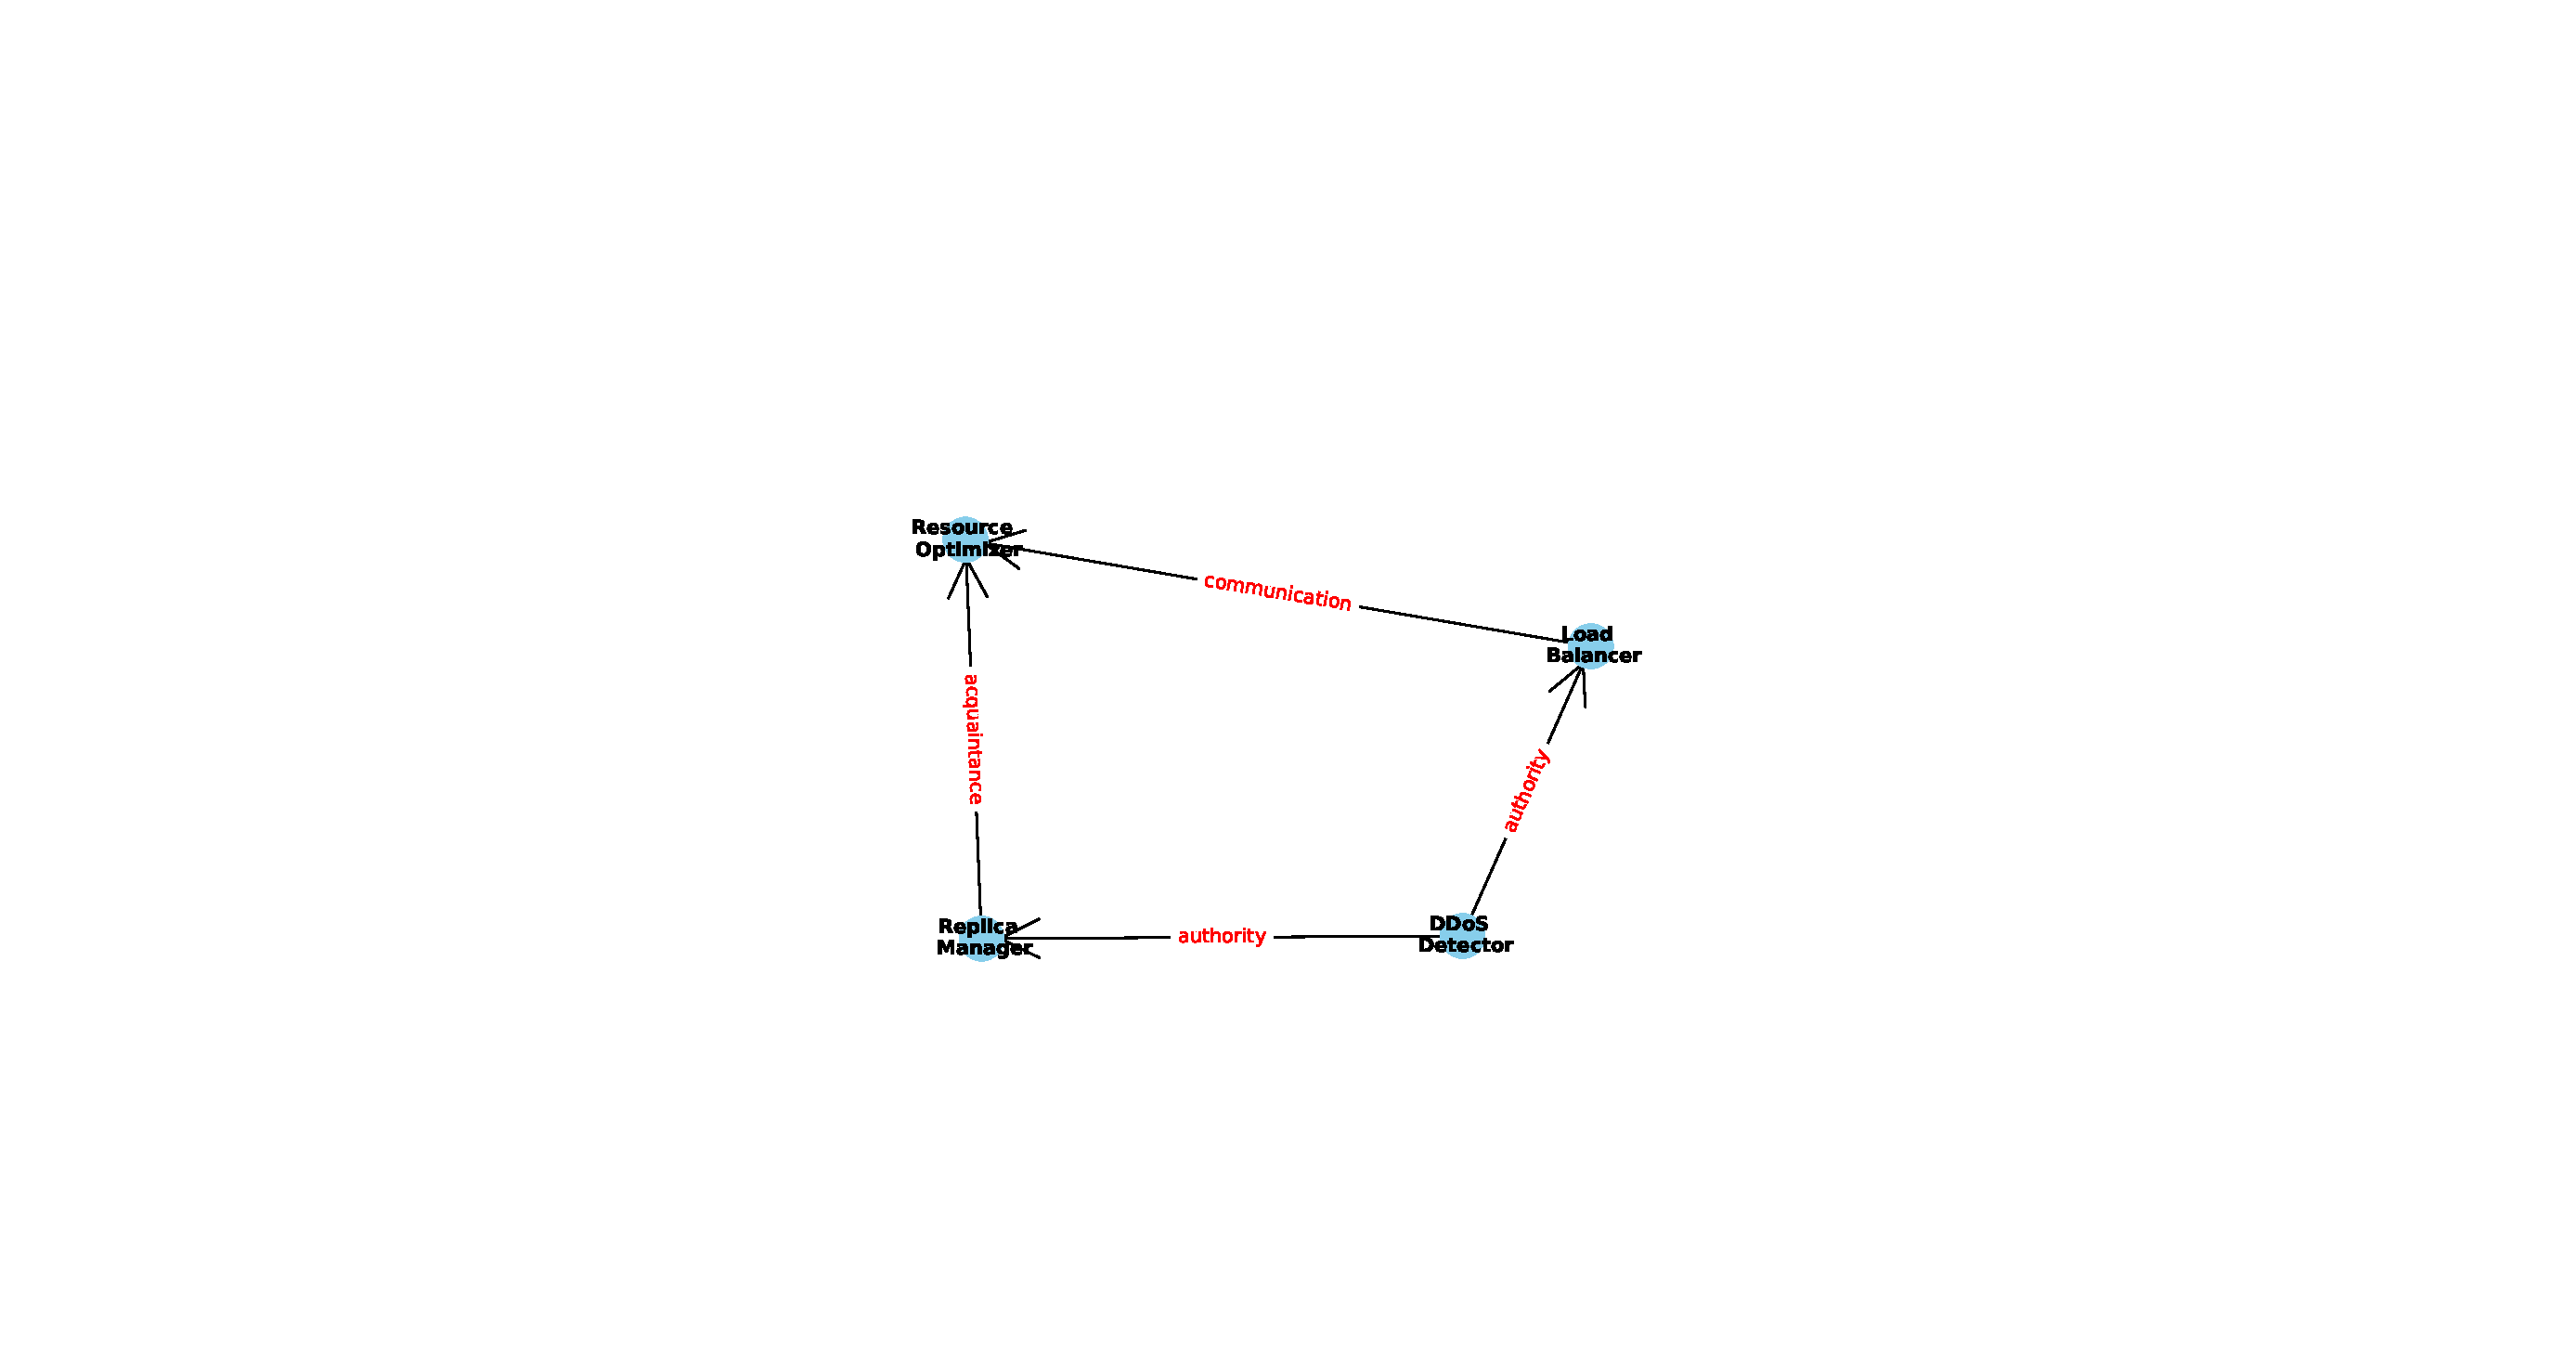
\includegraphics[trim=0cm 2cm 0cm 2cm, clip, width=0.5\textwidth]{figures/roles_graph.pdf}
    \caption{Exemple de graphe inter-agents déduit des trajectoires pendant une attaque DDoS : le \textit{DDoS Manager} détient l'autorité sur les autres agents et coordonne leurs réponses. Des relations supplémentaires capturent les communications observées (par exemple, Bottleneck et Resource Managers) et les liens de connaissance (par exemple, la connaissance entre Failure et Bottleneck Managers).}
    \label{fig:example_interaction_graph}
\end{figure}

%En considérant une fenêtre temporelle, nous pouvons générer un graphe basé sur les relations détectées, qui peut évoluer de manière dynamique lors de la fenêtre temporelle suivante, mettant en évidence les changements dans les modèles d'interaction.

% En outre, nous déterminons également les \textbf{modèles de coordination} qui visent à comprendre l'impact mutuel des actions d'un agent sur la trajectoire d'un autre agent  au fil du temps. Parmi les techniques d'exploration de modèles séquentiels, nous avons privilégié l'utilisation de l'algorithme \textit{PrefixSpan} pour identifier les séquences d'actions récurrentes entre les agents dans des scénarios spécifiques. Par exemple, les modèles peuvent montrer qu'un agent reporte ses actions à un autre dans des conditions adverses. Les séquences détectées peuvent être représentées sous forme de diagramme séquentiel illustrant la manière dont les agents interagissent au fil du temps, et montrant les relations causales et les dépendances dans la résolution des défis.



\subsection{Transfert}
\label{sec:transfert}

% Transfert : processus de transfert des comportements appris au cluster réel.
%  - récupérer les politiques entraînées dans un sous-module
%  - lancer les politiques entraînées avec l'état courant collecté
%  - appliquer les actions choisies par ces politiques via l'API K8s

%  - récupérer les politiques entraînées dans un sous-module

Dans cette phase, les politiques interagissent avec le cluster réel :
\begin{enumerate*}[label=\textbf{\arabic*)}, itemjoin={;\quad }]
    \item \textbf{Collecte d'états :} Des métriques en temps réel telles que l'utilisation du CPU, la consommation de mémoire, l'état des pods et le trafic réseau sont collectées à partir du serveur Prometheus~\cite{prometheus}
    \item \textbf{Exécution de la politique :} La politique $\pi_i$ de chaque agent calcule une action $a_t^i$ en fonction de l'état actuel $s_t$, en sélectionnant des ajustements tels que la mise à l'échelle des réplicas de pod pour un déploiement
    \item \textbf{Application des actions :} Les actions calculées sont envoyées sous forme de requêtes API, modifiant directement le déploiement.
\end{enumerate*}

Les agents du composant de transfert interagissent en permanence avec l'API Kubernetes, générant des états qui sont stockés dans la base de données du composant de modélisation. Au départ, une large fenêtre temporelle est utilisée pour collecter des traces représentatives afin de créer un jumeau numérique quasi réaliste du cluster Kubernetes. Ensuite, à intervalles réguliers plus courts, le composant de modélisation met à jour le jumeau numérique à l'aide des dernières données de trace. Ce processus itératif vise à garantir que les agents s'adaptent dynamiquement à la charge de travail.

\noindent \textit{Mécanismes de sécurité :} Afin de garantir le déploiement sécurisé des politiques, KARMA applique plusieurs mesures de protection à l'exécution. L'ampleur des actions est plafonnée afin d'éviter les comportements d'échelle extrêmes, et des mécanismes de repli permettent de revenir aux politiques KHPA standard si des états inattendus sont détectés. De plus, les politiques peuvent d'abord être testées dans le cadre de déploiements canaris, ce qui permet d'isoler leur effet avant leur déploiement complet. Les composants de surveillance évaluent en permanence les décisions des agents et déclenchent des alertes en cas d'anomalies.

%
% Les agents interagissent de manière transparente avec Kubernetes :
% \begin{enumerate*}[label={}, itemjoin={;\quad }]
%     \item Les actions sont appliquées aux déploiements via l'API
%     \item Les métriques en temps réel sont collectées à l'aide de Prometheus, garantissant ainsi des observations actualisées de l'état du cluster
%     \item KARMA fonctionne indépendamment des mécanismes HPA natifs de Kubernetes.
% \end{enumerate*}

% \

% \noindent Le cadre intègre une boucle de rétroaction :
% \begin{enumerate*}[label=\textbf{\arabic*)}, itemjoin={;\quad }]
%     \item Les métriques du cluster en direct sont utilisées pour mettre à jour le modèle de jumeau numérique.
%     \item Les agents sont régulièrement réentraînés sur ce modèle mis à jour afin d'affiner leurs politiques pour les nouveaux modèles de charge de travail ou les conditions défavorables.
%     \item Les politiques affinées sont redéployées sur le cluster, ce qui permet de maintenir une adaptabilité et une résilience élevées.
% \end{enumerate*}

% =======================================
\section{Configuration expérimentale}
\label{sec:experiments}
% Configuration expérimentale :
%  - Présenter les « services en chaîne »
%  - CybMASDE : présenter comme un moyen d'implémenter KARMA et présenter la configuration logicielle
%  - Configuration matérielle (pour l'entraînement et l'analyse)
%  - Protocole d'expérimentation et d'analyse (prend en compte une sorte d'étude d'ablation dans les baselines)
%  - Métriques d'évaluation
%  - Références : MA x (Org. Spec.)
%     - modèle sans spécifications organisationnelles avec 1 seul agent (état de l'art)
%     - modèle avec spécifications organisationnelles du modèle « fort » avec 1 seul agent (état de l'art ?)
%     - modèle sans spécifications organisationnelles avec plusieurs agents (état de l'art ?)
%     - modèle avec spécifications organisationnelles du modèle « faible » avec plusieurs agents
%     - modèle avec spécifications organisationnelles du modèle « fort » avec plusieurs agents

Cette section décrit la configuration expérimentale permettant d'évaluer la capacité de KARMA à combler les lacunes initialement définies.

\subsection{Description du cluster Kubernetes et de sa configuration}

L'environnement d'évaluation se compose d'un cluster Kubernetes simulant une architecture \textbf{Chained Services} (CS). Chaque service comprend un ensemble de microservices hébergés dans des pods et gérés par des déploiements. Par exemple, \autoref{fig:chained_services_graph} illustre la représentation graphique d'un cluster CS à quatre services. Nous avons envisagé d'utiliser un cluster caractérisé par les spécifications suivantes :

\begin{itemize}
    \item \textbf{Topologie :} Quatre services interconnectés en cours d'exécution, configurés pour émuler des conditions réelles, notamment des conflits de ressources, des goulots d'étranglement et des scénarios adversaires ;
    \item \textbf{Simulation de défaillance :} les goulots d'étranglement et les défaillances en cascade sont induits par des charges de travail gourmandes en ressources, tandis que les conditions adverses (par exemple, les attaques DDoS) sont émulées à l'aide de Locust~\cite{locust2021} et de scripts personnalisés basés sur le hasard ;
    \item \textbf{Nœuds de travail :} 1 nœud de travail avec 8 vCPU, 32 Go de RAM et une bande passante réseau de 1 Gbps. Cette configuration est adaptée à des fins de test sur des clusters de taille moyenne ;
    \item \textbf{Nœud d'entraînement :} 1 cluster à haute puissance de calcul composé de nœuds équipés de GPU NVIDIA Tesla V100 (16 Go), de processeurs Intel Xeon Platinum (2,3 GHz, 16 cœurs) et de 128 Go de RAM.
\end{itemize}

\begin{figure}[h!]
    \centering
    \hspace{-0,4cm}
    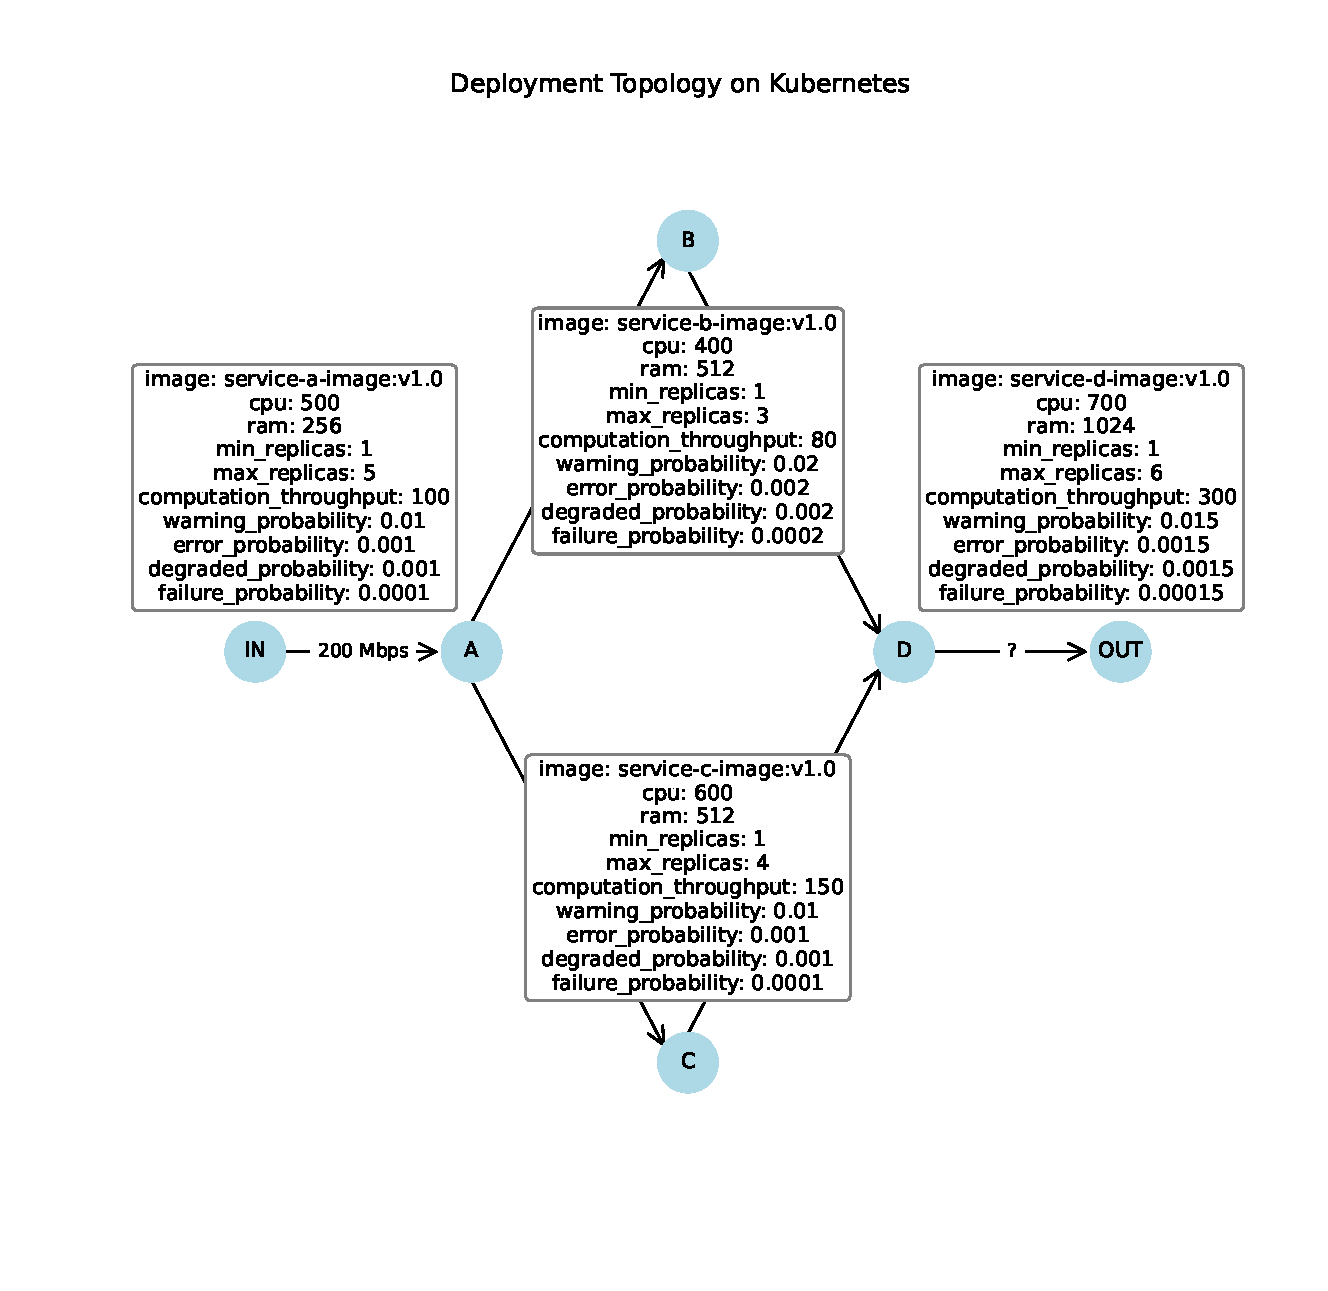
\includegraphics[trim=1.8cm 3.3cm 1.25cm 3.5cm, clip, width=0.5\textwidth]{figures/k8s_cluster_graph.pdf}
    \caption{Représentation graphique d'un cluster « Services en chaîne » avec quatre services}
    \label{fig:chained_services_graph}
\end{figure}

\subsection{Implémentation de KARMA avec CybMASDE}

% À FAIRE :
% - Présenter le framework CybMASDE
% - Scénario normal, scénario DDoS (augmentation ponctuelle du volume de données), scénario de défaillance (corruption ponctuelle des données), scénario de contention de ressources (priorisation), scénario mixte
% - Protocole d'expérimentation
%   - Baseline 1 : Agent unique sans spécifications organisationnelles souples
%   - Référence 2 : agent unique avec spécifications organisationnelles rigides
%   - Référence 3 : multi-agent sans spécifications organisationnelles
%   - Référence 4 : multi-agent avec spécifications organisationnelles

\footnotetext[2]{\label{lnk:footnote_2}Dans notre implémentation par défaut, $\alpha = 3$, $\sigma = 10$, $\kappa = 1$, $ch = 1$, poids des récompenses $(w_1, w_2, w_3, w_4, w_5) = (0,2, 0,2, 0,2, 0,2, 0,2)$, $Q_{\text{seuil}} = 30$ et $U_{\text{seuil}} = 90\%$.
Le code source de KARMA et d'autres hyperparamètres sont disponibles à l'adresse \url{https://github.com/julien6/KARMA}}.

Le framework KARMA s'appuie sur \textit{Cyber Multi-Agent System Development Environment}~\textsuperscript{\ref{lnk:footnote_2}} (CybMASDE), un framework MAS général d'aide à la conception qui s'intègre de manière transparente dans le framework KARMA.
Le framework comprend :
\begin{enumerate*}[label=\textbf{\arabic*)}, itemjoin={;\quad }]
    \item \textbf{Modélisation de jumeaux numériques :} un environnement de simulation reproduit le cluster Kubernetes à l'aide de traces réelles
    \item \textbf{Formation MARL :} \textit{MAPPO}~\cite{Yu2022} est utilisé pour former les agents dans l'environnement de jumeau numérique
    \item \textbf{Spécifications organisationnelles :} Les rôles et missions définis pour les agents guident le processus de formation, garantissant un comportement coordonné et explicable
    \item \textbf{Intégration du déploiement :} Les politiques formées interagissent avec l'API Kubernetes pour ajuster les réplicas de pods en temps réel.
\end{enumerate*}

\subsection{Rôles et missions pour la résilience opérationnelle}

\noindent Conformément au $\mathcal{M}OISE^+$~\cite{hubner2002moise} et aux principes architecturaux de l'AICA~\cite{kott2018autonomous}, nous avons mis en œuvre quatre rôles afin de traiter un facteur de dégradation spécifique dans une QoS.
% et définit les actions autorisées des agents.
Chaque rôle est associé à une mission, contenant un seul sous-objectif basé sur des métriques.

\noindent \paragraph{\textbf{Gestionnaire des goulots d'étranglement}} 
%
Le rôle du \textit{gestionnaire des goulots d'étranglement} consiste à surveiller les services afin de détecter les goulots d'étranglement causés par des flux de trafic déséquilibrés. Il repose sur des règles suivant ces indicateurs :
\begin{enumerate*}[label={}, itemjoin={;\quad }]
    \item \( T_{\text{in}}^i \): Trafic entrant pour le service \( i \) (Kbps)
    \item \( T_{\text{out}}^i \): Trafic sortant pour le service \( i \)
    \item \( Q_{\text{pending}}^i \): Demandes en attente pour le service \( i \).
\end{enumerate*}
Un goulot d'étranglement est détecté si : $Q_{\text{en attente}}^i > Q_{\text{seuil}} \quad \text{ou} \quad T_{\text{in}}^i > \alpha \cdot T_{\text{out}}^i$
où \( Q_{\text{threshold}} \) est le seuil critique de la file d'attente et \( \alpha > 1 \) est un facteur d'amplification.

La mission associée vise à minimiser la taille de la file d'attente en attente afin d'éliminer les goulots d'étranglement. La fonction de récompense est définie comme suit : $R_{\text{bottleneck}} = - \sum_{i} Q_{\text{pending}}^i$
Les agents sont récompensés pour avoir réduit les demandes en attente, optimisant ainsi le débit~\cite{burns2016borg}.

\noindent \paragraph{\textbf{Gestionnaire DDoS}}

Le rôle du \textit{DDoS Manager} consiste à identifier les attaques DDoS en analysant les anomalies du trafic :
\begin{enumerate*}[label={}, itemjoin={;\quad }]
    \item \( R_{\text{rate}} \): Taux de requêtes entrantes pour le cluster.
    \item \( L_{\text{avg}} \): Latence moyenne observée.
    \item \( \Delta T \): Variation du volume de trafic sur une période \( t \).
\end{enumerate*}
Une attaque DDoS est détectée lorsque :
$R_{\text{rate}} > R_{\text{threshold}} \quad \text{et} \quad \Delta T > \Delta T_{\text{threshold}}$
où \( R_{\text{seuil}} \) est un seuil critique de trafic.

La mission associée consiste à isoler les services affectés afin de minimiser les temps d'arrêt à l'aide de la fonction de récompense suivante :
$R_{\text{ddos}} = - \left( \text{DownTime} \cdot w_{\text{d}} + L_{\text{avg}} \cdot w_{\text{l}} \right)$
où \( w_{\text{d}} \) et \( w_{\text{l}} \) sont les pondérations pour les temps d'indisponibilité et la latence, respectivement~\cite{Liu2018}.

\noindent \paragraph{\textbf{Gestionnaire des pannes}}

Le rôle du \textit{Gestionnaire des défaillances} consiste à surveiller l'état des pods et à éliminer les pods défaillants selon la règle suivante :
\begin{enumerate*}[label={}, itemjoin={;\quad }]
    \item \( F_{\text{fail}}^i \): Nombre de défaillances pour le pod \( i \)
    \item \( S_{\text{status}}^i \): Statut du pod \( i \) (par exemple, \textit{CrashLoopBackOff}).
\end{enumerate*}
Une défaillance de pod est détectée si :
$F_{\text{fail}}^i > F_{\text{threshold}}$
où \( F_{\text{threshold}} \) est le nombre maximal de défaillances tolérées.

La mission associée minimise les temps d'arrêt causés par des défaillances répétées à l'aide de cette fonction de récompense :
$R_{\text{échec}} = - \sum_{i} T_{\text{temps d'indisponibilité}}^i$
Les agents sont incités à éliminer rapidement les services défaillants et à les redémarrer.

\noindent \paragraph{\textbf{Gestionnaire de ressources}}

Le rôle du \textit{gestionnaire de ressources} consiste à hiérarchiser les services critiques en cas de conflit d'accès aux ressources. Les règles sont basées sur :
\begin{enumerate*}[label={}, itemjoin={;\quad }]
    \item \( U_{\text{cpu}}^i \): utilisation du processeur par le service \( i \)
    \item \( U_{\text{mem}}^i \): utilisation de la mémoire du service \( i \)
    \item \( P_{\text{priority}}^i \): niveau de priorité du service \( i \) (critique, normal, faible).
\end{enumerate*}
Une contention est détectée si l'utilisation totale du CPU dépasse un seuil :
$U_{\text{cpu}}^{\text{total}} > U_{\text{threshold}}$
Les services non critiques sont réduits afin de libérer des ressources :
$\text{Réplicas}_{\text{nouveau}}^i = \max\left( \text{Réplicas}_{\text{actuel}}^i - \delta, 1 \right)$

La mission associée garantit les services critiques en équilibrant l'utilisation des ressources à l'aide de cette fonction de récompense :
$R_{\text{resource}} = - \sum_{i \in \text{Critical}} \left( U_{\text{cpu}}^i + U_{\text{mem}}^i \right)$
Les agents sont récompensés pour avoir donné la priorité aux services tout en maintenant une utilisation efficace des ressources~\cite{shahrad2020resource}.

\

\subsection{Protocole expérimental}

\noindent Afin d'évaluer les performances de KARMA dans la résolution des six lacunes, nous proposons de comparer les scénarios de référence entre eux.

\paragraph{\textbf{Intégration et évaluation de clusters réels}}

KARMA associe la simulation à l'interaction avec un cluster réel en créant un jumeau numérique à partir de traces Kubernetes réelles. Les politiques formées sont déployées via l'API Kubernetes, influençant le cluster réel, tandis que de nouvelles traces affinent la simulation. Cela garantit une applicabilité dans le monde réel avec une formation des agents dans un environnement sûr.

\paragraph{\textbf{Scénarios expérimentaux}}

\noindent Cinq scénarios expérimentaux sont définis pour simuler les facteurs clés qui influent sur la résilience opérationnelle dans Kubernetes :
%
\begin{enumerate*}[label=\textbf{\arabic*)}, itemjoin={;\quad }]
    \item \textbf{Résolution des goulots d'étranglement :} Simule des scénarios dans lesquels les services en amont surchargent les services en aval afin de maximiser le débit en adaptant dynamiquement le nombre de réplicas
    \item \textbf{Attaque DDoS :} Modélise une augmentation soudaine du trafic visant à perturber les services critiques afin de détecter l'attaque, d'isoler les services affectés et de minimiser les temps d'arrêt~\cite{Liu2018}
    \item \textbf{Pannes de pod :} Des pannes de pod sont déclenchées pour évaluer la capacité du système à restaurer les services affectés~\cite{burns2016borg}
    \item \textbf{Contention des ressources :} Simule une forte demande en ressources, nécessitant une hiérarchisation dynamique des services critiques afin de maintenir la fonctionnalité globale du cluster~\cite{Vhatkar2022}
    \item \textbf{Scénario mixte :} Combine tous les scénarios pour évaluer l'adaptabilité et la résilience du système.
\end{enumerate*}

\paragraph{\textbf{Références issues de la littérature}}
%
\noindent Nous avons sélectionné trois systèmes HPA comme références :
\begin{enumerate*}[label=\textbf{\arabic*)}, itemjoin={;\quad }]
    \item \textbf{AWARE :} un système basé sur le RL qui équilibre le temps de réponse et le débit~\cite{aware2023}
    \item \textbf{Gym-HPA :} un environnement RL pour expérimenter divers algorithmes RL en simulation~\cite{gymhpa2022}
    \item \textbf{Rlad-core}~\cite{Rossi2019} Un simulateur basé sur le RL qui utilise des techniques d'apprentissage automatique pour faire évoluer les services, notamment le Q-learning et les algorithmes basés sur des modèles.
\end{enumerate*}

Ces références ont été testées dans les cinq mêmes scénarios à l'aide du code source lorsqu'il était disponible.

\paragraph{\textbf{Références en tant qu'études d'ablation}}

\noindent Afin d'isoler les contributions des composants de KARMA, des études d'ablation ont été réalisées selon les configurations suivantes :
%
\begin{itemize}
    \item \textbf{Avec/sans MLP :} Évalue l'impact de l'utilisation d'un transitionneur basé sur un MLP pour la modélisation de jumeaux numériques.
    \item \textbf{Avec/sans spécifications organisationnelles :} Teste les contraintes organisationnelles strictes et souples pendant la formation :
        \begin{itemize}
            \item \textit{Contraintes strictes :} Applique strictement les rôles et les missions.
            \item \textit{Contraintes souples :} Autoriser les actions exploratoires avec des récompenses basées sur les spécifications organisationnelles.
        \end{itemize}
    \item \textbf{Multi-agent vs mono-agent :} Comparaison d'une configuration multi-agent avec une configuration mono-agent de référence.
\end{itemize}

\paragraph{\textbf{Indicateurs de performance}}

\noindent Pour chaque scénario et référence, les indicateurs suivants sont collectés :
%
\begin{enumerate*}[label=\textbf{\arabic*)}, itemjoin={;\quad }]
    \item \textbf{Résilience opérationnelle :} Basée sur la récompense globale issue du taux de réussite (\%), le ratio de requêtes en attente (\%), la latence moyenne (ms)
    \item \textbf{Robustesse face aux attaques :} Basée sur l'écart type de la récompense et le temps de récupération après une attaque DDoS (s), pourcentage de services restant disponibles (\%)
    \item \textbf{Précision du jumeau numérique :} Basée sur la précision du modèle de transition (\%), calculée comme le rapport entre les performances réelles du cluster et celles de la simulation
    \item \textbf{Génération automatisée de MAS :} Basée sur le temps de convergence de l'entraînement (nombre d'épisodes)
    \item \textbf{Adaptabilité :} Basée sur la variance de l'écart type de la récompense sur les épisodes d'entraînement dans tous les scénarios (\%)
    \item \textbf{Explicabilité :} Basée sur l'alignement des comportements avec les rôles/missions lorsqu'ils sont donnés (\%), et sur l'évaluation qualitative du regroupement des trajectoires.
\end{enumerate*}



\section{Résultats et discussion}
\label{sec:results}

Cette section analyse les performances de KARMA dans la résolution des six lacunes identifiées.


\subsection{Lacune 1 : Résilience opérationnelle}
La résilience opérationnelle évalue la capacité du système à gérer les défaillances et à maintenir une qualité de service élevée.
\begin{table}[h]
    \centering
    \caption{Indicateurs de résilience opérationnelle dans tous les scénarios.}
    \label{tab:operational_resilience}{\footnotesize
    \begin{tabular}{>{\raggedright\arraybackslash}m{2.7cm}>{\centering\arraybackslash}m{1.5cm}>{\centering\arraybackslash}m{1.5cm}>{\centering\arraybackslash}m{1.5cm}}
        \hline
        \textbf{Référence} & \textbf{Taux de réussite (\%)} & \textbf{Conformité en matière de latence (\%)} & \textbf{Demandes en attente (\%)} \\
        \hline
        KHPA & 64,8 & 58,1 & 20,7 \\
        Gym-HPA & 73,1 & 65,7 & 20,8 \\
        Rlad-core & 77,4 & 70,1 & 15,9 \\
        AWARE & 80,6 & 73,8 & 13,3 \\
        Agent unique sans spécificité organique & 72,6 & 65,4 & 17,0 \\
        Agent unique avec spécification organisationnelle stricte & 80,8 & 72,5 & 15,4 \\
        Multi-agent sans spécification organisationnelle & 87,7 & 81,5 & 9,3 \\
        Multi-agent avec spécifications organisationnelles souples & 82,0 & 74,7 & 15,0 \\
        \textbf{Multi-agents avec spécifications organisationnelles rigides (KARMA)} & \textbf{90,9} & \textbf{85,7} & \textbf{5,9} \\
        \hline
    \end{tabular}}
\end{table}
%
\autoref{tab:operational_resilience} présente une comparaison entre KARMA et les références existantes. Les résultats montrent que KARMA atteint le taux de réussite le plus élevé (\textbf{90,9\%}), surpassant toutes les références, y compris AWARE (80,6\%) et Rlad-core (\textbf{77,4\%}). De même, la conformité de KARMA en matière de latence est la plus élevée avec \textbf{85,7\%}, tandis que le taux de requêtes en attente le plus bas (\textbf{5,9\%}) suggère une gestion efficace des variations de charge de travail.

\noindent \textit{Remarque statistique :} Toutes les valeurs indiquées représentent la moyenne de 10 évaluations indépendantes. Bien que cela ne soit pas indiqué dans les tableaux par souci de concision, l'écart type entre les évaluations est resté faible ($\pm$1,8\% pour le taux de réussite et $\pm$2,1 ms pour la latence dans le scénario mixte), ce qui indique des résultats robustes.

Les performances de KARMA découlent de sa coordination multi-agents structurée, qui répartit de manière optimale les ressources en fonction des contextes de défaillance, évitant ainsi les actions de mise à l'échelle redondantes ou conflictuelles, problèmes courants dans les autoscalers basés sur le RL à agent unique.
%
Les autoscalers réactifs basés sur des seuils, tels que KHPA et Gym-HPA, ont du mal à gérer les charges de travail dynamiques, ce qui entraîne une augmentation des demandes en attente et une baisse des taux de réussite. AWARE et Rlad-core améliorent le temps de réponse et le débit, mais ne disposent pas d'une coordination multi-agents, ce qui se traduit par des réactions plus lentes dans les scénarios adversaires. Les systèmes à agent unique sans spécifications organisationnelles souffrent d'une allocation inefficace des ressources, tandis que les systèmes à agent unique avec spécifications organisationnelles rigides bénéficient d'une prise de décision structurée, mais manquent encore de coordination distribuée.

La coordination basée sur les rôles de KARMA minimise les inefficacités et améliore la stabilité des décisions. Sa décomposition hiérarchique des objectifs permet des décisions indépendantes mais complémentaires, ce qui se traduit par une mise à l'échelle automatique plus résiliente.

Les résultats soulignent également la valeur des contraintes organisationnelles. Les systèmes multi-agents avec des contraintes souples (taux de réussite de 82,0 %) surpassent les approches à agent unique, mais les contraintes strictes de KARMA obtiennent les meilleurs résultats, éliminant les comportements conflictuels des agents et optimisant la mise à l'échelle.



\subsection{Écart 2 : Conditions adverses}

Les conditions adverses évaluent la robustesse du système face à des scénarios perturbateurs tels que les attaques DDoS.
\begin{table}[h]
    \centering
    \caption{Performances dans un scénario DDoS.}
    \label{tab:adversarial_conditions}{
        \footnotesize
    \begin{tabular}{>{\raggedright\arraybackslash}m{3.6cm}>{\centering\arraybackslash}m{1.8cm}>{\centering\arraybackslash}m{2cm}}
        \hline
        \textbf{Référence} & \textbf{Temps de récupération (s)} & \textbf{Disponibilité du service (\%)} \\
        \hline
        KHPA & 80,7 & 65,6 \\
        Gym-HPA & 66,2 & 72,6 \\
        Rlad-core & 37,4 & 78,3 \\
        AWARE & 49,5 & 83,6 \\
        Agent unique sans spécificité organique & 60,3 & 72,4 \\
        Agent unique avec spécificité organisationnelle dure & 48,5 & 77,5 \\
        Multi-agent sans spécification organisationnelle & 43,5 & 82,0 \\
        Multi-agent avec spécifications organisationnelles souples & 38,8 & 86,0 \\
        \textbf{Multi-agent avec spécifications organisationnelles strictes (KARMA)} & \textbf{33,0} & \textbf{90,7} \\
        \hline
    \end{tabular}}
\end{table}
%
\autoref{tab:adversarial_conditions} compare les temps de récupération et la disponibilité du service dans le scénario \textit{Attaque DDoS}. KARMA atteint le temps de récupération le plus rapide (\textbf{33,0 s}), surpassant AWARE (\textbf{38,8 s}) et Rlad-core (\textbf{43,5 s}). Il garantit également une bonne disponibilité du service à \textbf{90,7\%}, réduisant ainsi les temps d'indisponibilité par rapport à AWARE (\textbf{83,6\%}).

Les autoscalers traditionnels tels que KHPA et Gym-HPA s'appuient sur une mise à l'échelle réactive basée sur des seuils, ce qui entraîne une récupération plus lente et une disponibilité du service plus faible en cas d'attaques. Les méthodes basées sur le RL telles que Rlad-core et AWARE améliorent la résilience, mais manquent de coordination structurée, ce qui les rend moins efficaces contre les pics adverses. Les approches à agent unique ont du mal à trouver un équilibre entre l'atténuation des attaques et l'optimisation des ressources, tandis que les modèles multi-agents avec des contraintes souples permettent des actions exploratoires qui retardent parfois les réponses optimales.

L'apprentissage proactif et la coordination structurée de KARMA lui permettent d'anticiper les attaques plutôt que de réagir après une dégradation. Des contraintes explicites basées sur les rôles garantissent que les agents donnent la priorité aux actions de mise à l'échelle critiques, ce qui se traduit par une atténuation plus rapide et une disponibilité plus élevée. Ces résultats soulignent l'efficacité de l'apprentissage structuré multi-agents dans la mise à l'échelle automatique sensible à la sécurité, où les méthodes traditionnelles présentent une adaptation plus lente et des temps d'arrêt prolongés.


\subsection{Lacune 3 : Modélisation des jumeaux numériques}

\begin{table}[h]
    \centering
    \caption{Précision des modèles de transition dans tous les scénarios.}
    \label{tab:digital_twin_accuracy}{
        \footnotesize
    \begin{tabular}{>{\raggedright\arraybackslash}m{6cm}>{\centering\arraybackslash}m{2cm}}
        \hline
        \textbf{Référence} & \textbf{Précision (\%)} \\
        \hline
        Sans modèle de transition MLP & 83,5 \\
        \textbf{Avec modèle de transition MLP (KARMA)} & \textbf{94,9} \\
        \hline
    \end{tabular}}
\end{table}
%
La précision du modèle de jumeau numérique est essentielle pour former des agents dans des conditions réalistes.
\autoref{tab:digital_twin_accuracy} compare la précision de différents modèles de jumeaux numériques. Les résultats montrent que KARMA atteint une précision de \textbf{94,9\%}, surpassant le modèle non MLP (\textbf{83,5\%}), qui peine à généraliser.

Cette amélioration découle de la capacité du modèle MLP à saisir les dépendances non linéaires entre les fluctuations de la charge de travail, l'allocation des ressources et les actions de mise à l'échelle. Sans cette fonctionnalité, le système ne parvient pas à modéliser avec précision les comportements complexes des clusters.
%
En exploitant un réseau neuronal pour la modélisation des transitions, KARMA garantit un jumeau numérique plus fiable, permettant aux agents de s'entraîner dans des conditions proches de la réalité. Cela réduit le risque de mauvaises décisions lors du transfert des politiques vers la production, renforçant ainsi l'importance des simulations haute fidélité.



\subsection{Lacune 4 : Génération automatisée de MAS}

L'efficacité de la génération d'un MAS est évaluée en termes de temps de convergence et de surcoût de formation. \autoref{tab:mas_generation_efficiency} présente les résultats pour les différents scénarios concernés, tandis que \autoref{fig:learning_curves} montre les courbes d'apprentissage dans le scénario mixte sur 2000 épisodes.

\begin{table}[h]
    \centering
    \caption{Efficacité de la génération de MAS dans tous les scénarios.}
    \label{tab:mas_generation_efficiency}{
        \footnotesize
    \begin{tabular}{>{\raggedright\arraybackslash}m{3.5cm}>{\centering\arraybackslash}m{2cm}>{\centering\arraybackslash}m{2cm}}
        \hline
        \textbf{Référence} & \textbf{Temps de convergence (épisodes)} & \textbf{Charge de formation (heures)} \\
        \hline
        Multi-agents sans spécifications organisationnelles & 1800 & 4 \\
        \textbf{Multi-agents avec spécifications organisationnelles strictes (KARMA)} & \textbf{950} & \textbf{1,5} \\
        \hline
    \end{tabular}}
\end{table}

L'apprentissage guidé par les rôles réduit l'espace de recherche des politiques optimales, ce qui permet une convergence plus rapide et une réduction des coûts de calcul. Ces gains d'efficacité sont particulièrement importants pour adapter les solutions MAS à des environnements complexes.

Les courbes d'apprentissage dans \autoref{fig:learning_curves} montrent que KARMA atteint une convergence stable beaucoup plus rapidement que la référence sans spécifications organisationnelles. À l'épisode 950, KARMA présente une variance minimale dans les récompenses cumulées, tandis que la référence nécessite près du double d'épisodes (1800) pour atteindre des performances comparables. Cela souligne le rôle des contraintes organisationnelles dans l'orientation des agents vers des politiques efficaces, réduisant ainsi les coûts d'exploration.

\noindent \textit{Discussion sur la charge :} La phase d'entraînement de KARMA a nécessité environ 1,5 heure sur une machine haute performance équipée d'un GPU (Tesla V100, 16 Go) et de 16 cœurs CPU, avec une convergence en moins de 1 000 épisodes. Au moment de l'inférence, la politique de chaque agent produit des décisions en moins de 30 ms, avec une empreinte mémoire négligeable (moins de 50 Mo par agent).

\autoref{tab:mas_generation_efficiency} montre une réduction du \textit{temps de convergence} d'environ \textbf{47\%} par rapport à Multi-Agent w/o Org. Spec., démontrant l'efficacité de l'apprentissage guidé par les rôles pour minimiser les explorations inutiles. De plus, la \textit{surcharge de formation} est réduite de \textbf{62,5\%}, ce qui démontre une meilleure praticité pour les systèmes à grande échelle où les ressources informatiques constituent un facteur limitant.

\begin{figure}[h!]
    \centering
    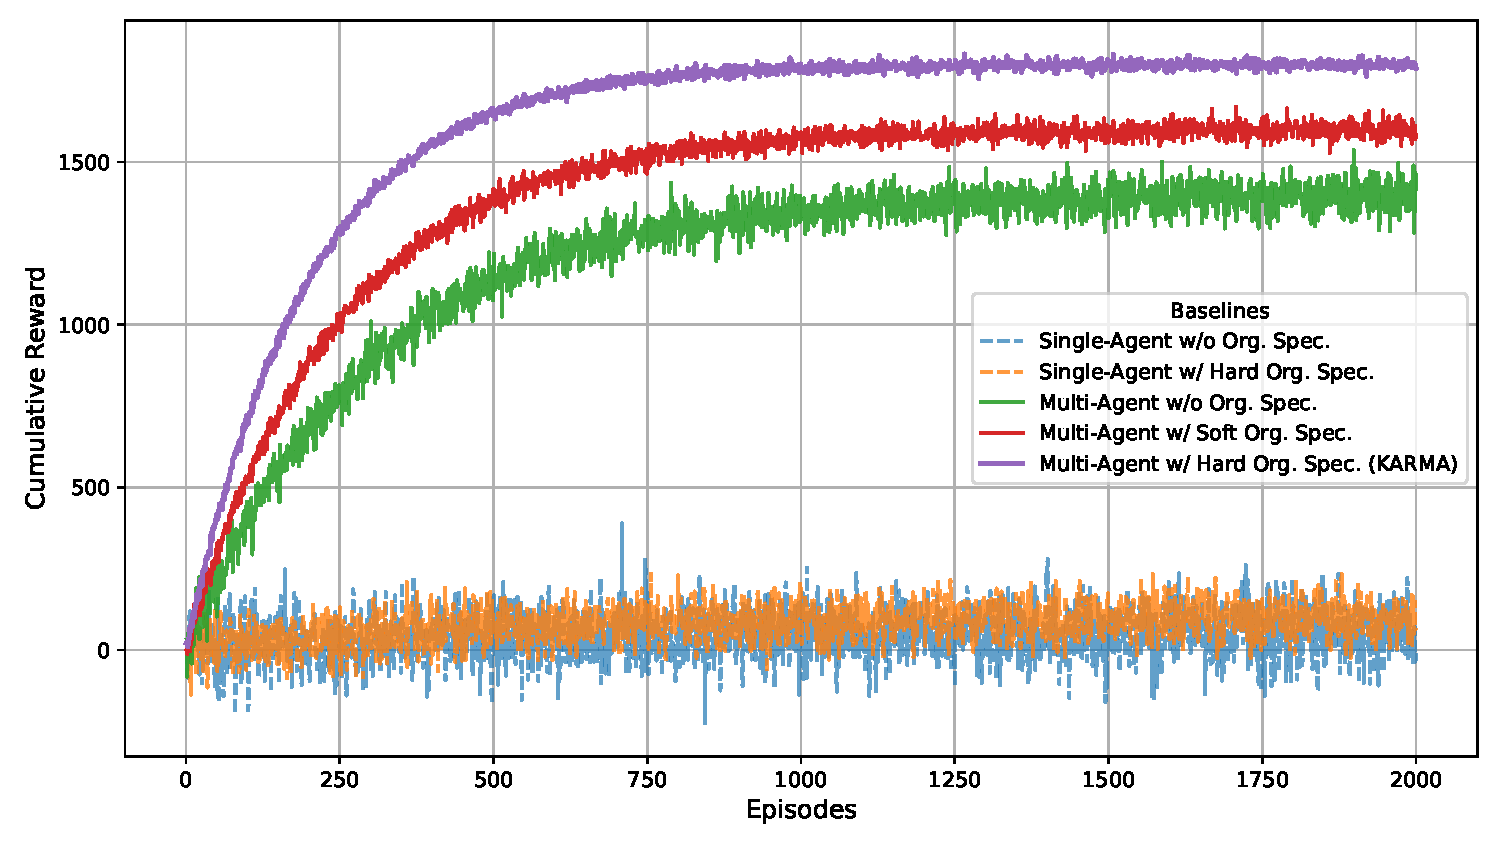
\includegraphics[width=0.49\textwidth]{figures/learning_curves.pdf}
    \caption{Courbes d'apprentissage entre les lignes de base pour le scénario mixte sur 2000 épisodes.}
    \label{fig:learning_curves}
\end{figure}


\subsection{Écart 5 : Adaptabilité}

L'adaptabilité évalue la capacité du système à maintenir ses performances sous des charges de travail dynamiques dans différents scénarios.
\begin{table}[h]
    \centering
    \caption{Comparaison de l'adaptabilité dans le scénario mixte.}
    \label{tab:adaptability_comparison}{
    \footnotesize
    \begin{tabular}{>{\raggedright\arraybackslash}m{5cm}>{\centering\arraybackslash}m{3cm}}
        \hline
        \textbf{Référence} & \textbf{Récompense s.t.d (\%)} \\
        \hline
        Agent unique sans spécification organisationnelle & 11,1 \\
        Agent unique avec spécifications organisationnelles strictes & 11,1 \\
        Multi-agents sans spécifications organisationnelles & 10,7 \\
        Multi-agent avec spécifications organisationnelles souples & 9,0 \\
        \textbf{Multi-agent avec spécifications organisationnelles rigides (KARMA)} & \textbf{5,3} \\
        \hline
    \end{tabular}}
\end{table}
%
\autoref{tab:adaptability_comparison} montre que KARMA obtient l'écart type de récompense le plus faible (\textbf{5,3\%}), ce qui indique une performance très stable, surpassant Multi-Agent avec spécifications organisationnelles souples (\textbf{9,0\%}) et Multi-Agent sans spécifications organisationnelles (\textbf{10,7\%}).

Dans le \textit{scénario mixte}, les modèles à agent unique présentent une variance plus élevée, car ils doivent équilibrer plusieurs objectifs concurrents sans spécialisation. Les approches multi-agents améliorent l'adaptabilité, mais sans coordination structurée, les fluctuations persistent. L'utilisation de contraintes organisationnelles souples stabilise les performances, même si certaines variations exploratoires persistent.

L'apprentissage par renforcement hiérarchique de KARMA garantit une variabilité moindre en décomposant l'objectif global en sous-objectifs spécialisés. Cette approche structurée permet aux agents de se concentrer sur des objectifs bien définis, ce qui réduit les décisions contradictoires et améliore la stabilité globale.
%
Ces résultats soulignent l'importance des cadres d'apprentissage structurés dans l'auto-scaling. En imposant des spécialisations claires aux agents, KARMA améliore l'adaptabilité et garantit des performances résilientes dans des conditions de charge de travail imprévisibles.


\subsection{Écart 6 : Expliquabilité}
\label{subsec:gap_explainability}

L'explicabilité est évaluée qualitativement à travers le regroupement des trajectoires et quantitativement à travers l'alignement des comportements des agents avec des rôles et des missions prédéfinis.
\noindent \autoref{fig:trajectory_clustering_hrl} illustre le dendrogramme généré par le regroupement hiérarchique des séquences d'actions des agents avec les quatre rôles appliqués, en utilisant DTW comme mesure de similarité. La figure met en évidence l'émergence de quatre groupes distincts, chacun correspondant à un rôle organisationnel spécifique, démontrant la capacité des comportements des agents à s'aligner sur les rôles prédéfinis.

\begin{figure}[h!]
    \centering
    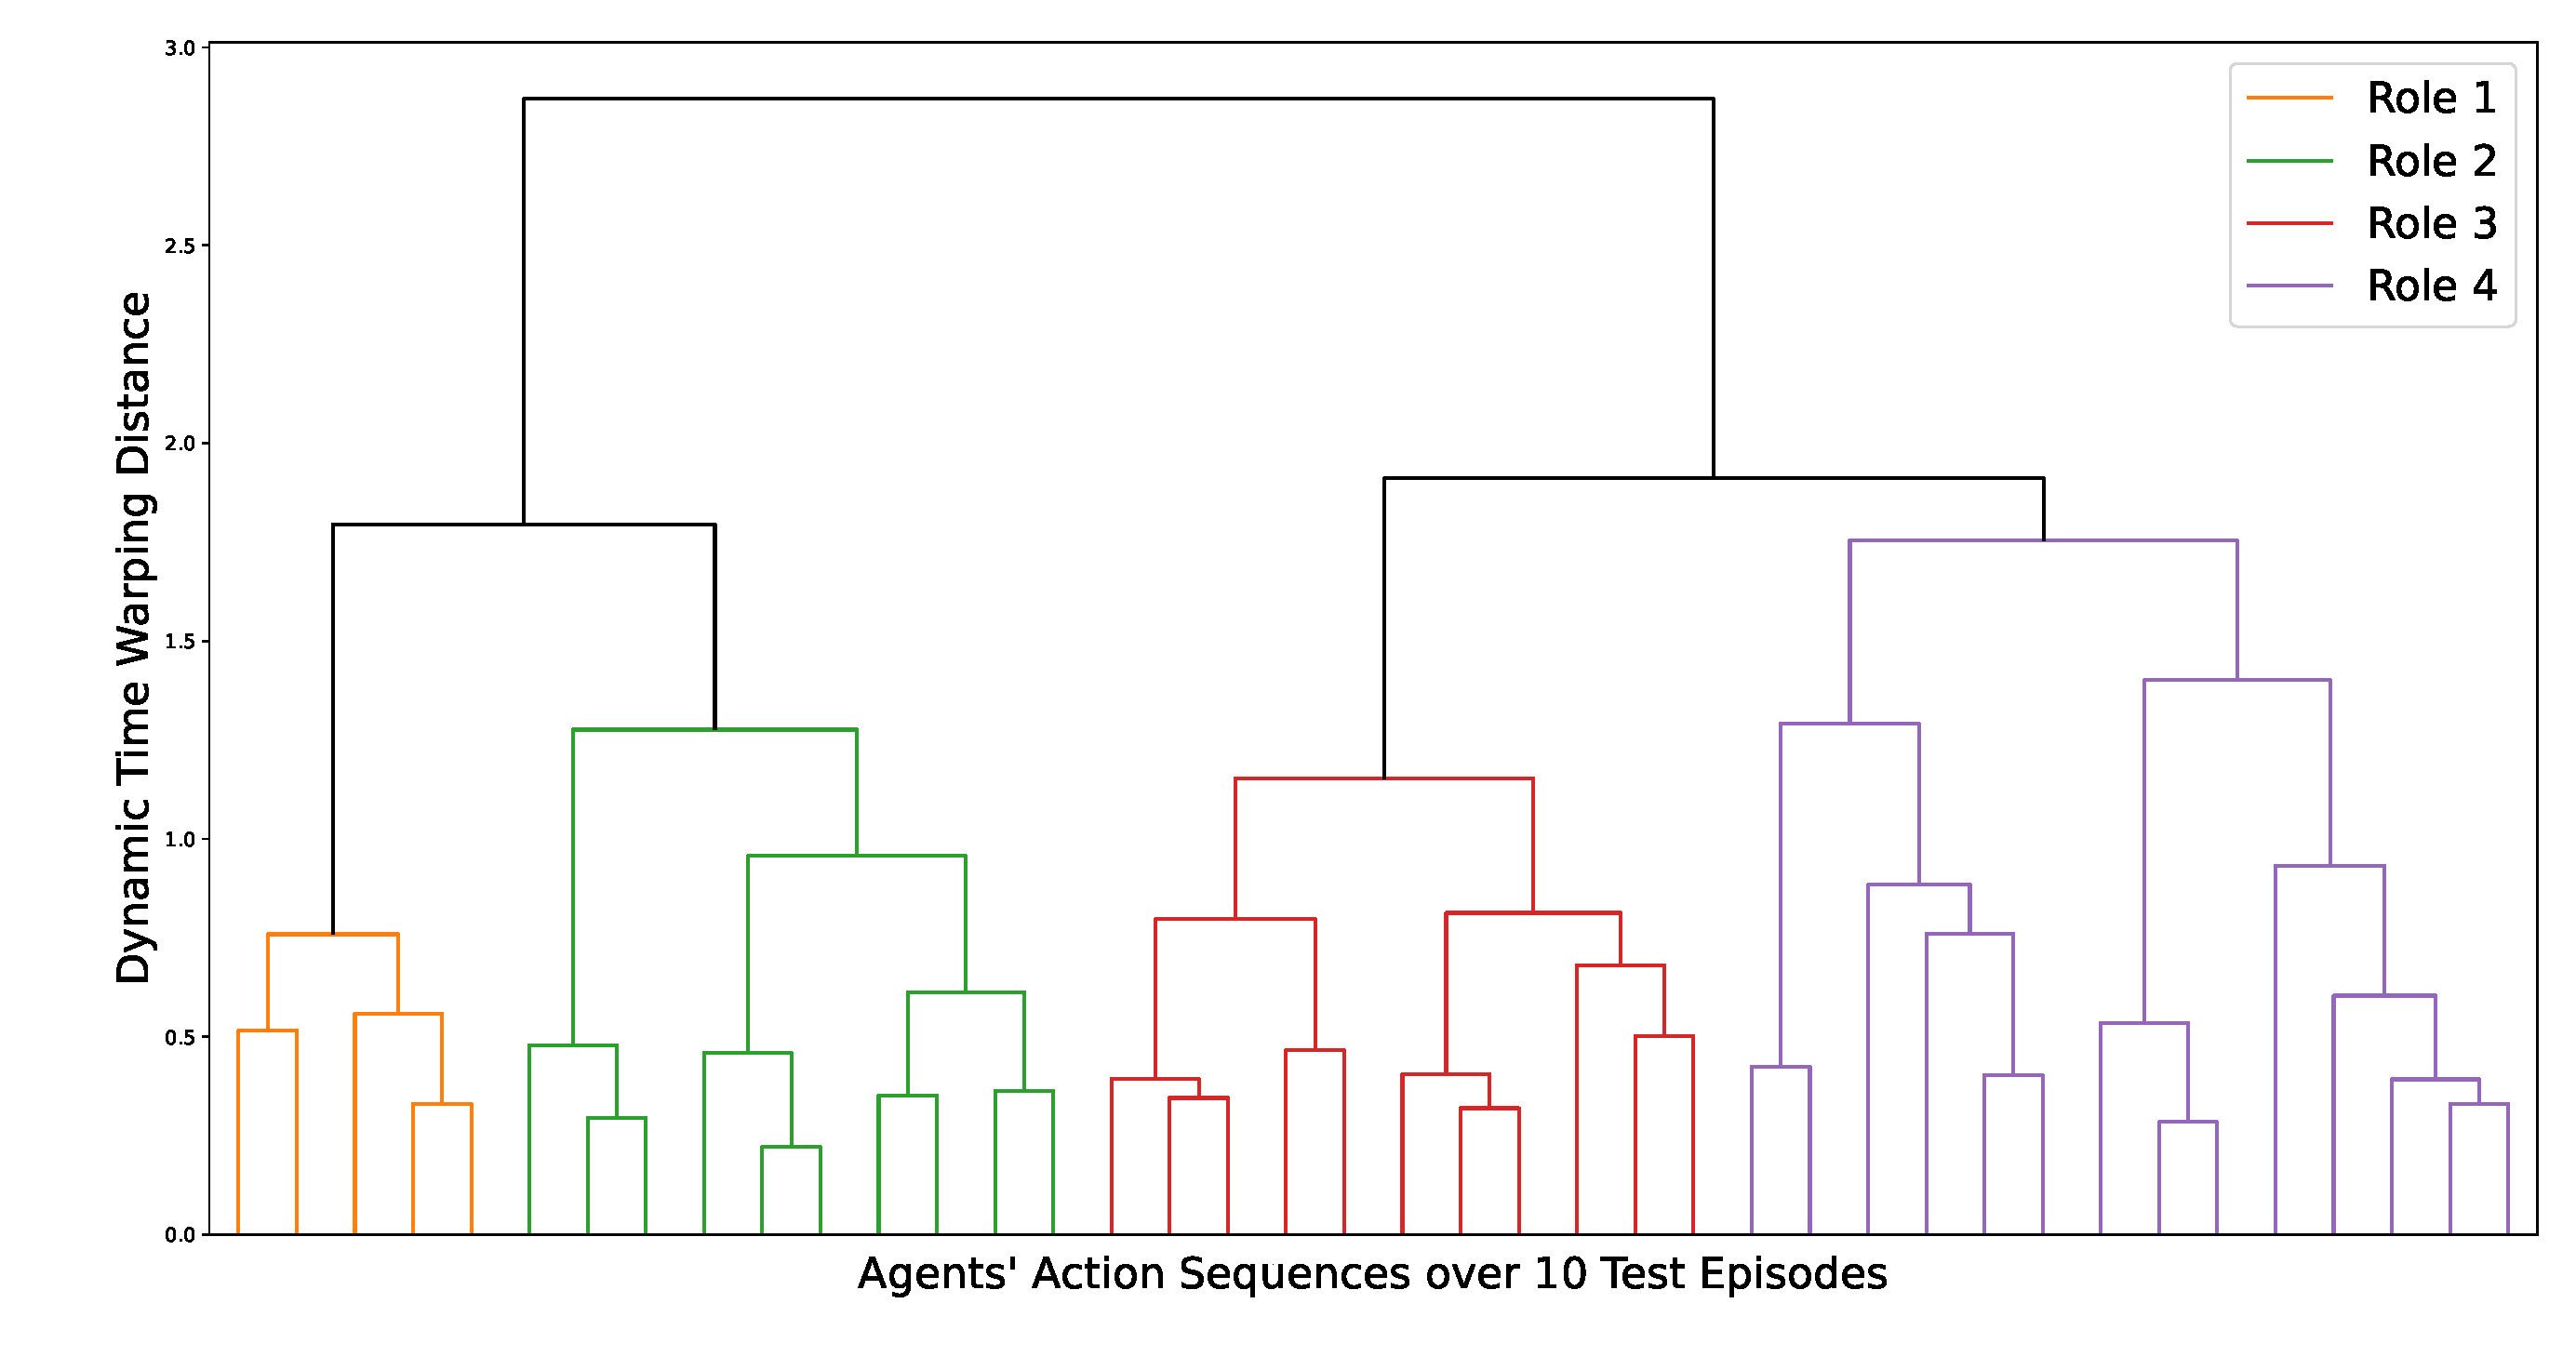
\includegraphics[width=0.49\textwidth]{figures/role_hierarchical_clustering.pdf}
    \caption{Dendrogramme obtenu après regroupement hiérarchique des trajectoires des agents pour l'inférence des rôles dans le scénario mixte.}
    \label{fig:trajectory_clustering_hrl}
\end{figure}

\begin{table}[h!]
    \centering
    \caption{Alignement des agents avec leurs rôles et missions.}
    \label{tab:alignment}
    {\footnotesize
    \begin{tabular}{>{\raggedright\arraybackslash}m{4.1cm}>{\centering\arraybackslash}m{1.5cm}>
    {\centering\arraybackslash}m{1.5cm}}
    \toprule
    \textbf{Référence} & \textbf{Score d'alignement (\%)} & \textbf{Pureté du regroupement (\%)} \\
    \midrule
    Multi-agents sans spécification organisationnelle & $\emptyset$ & 62,7 \\
    Multi-agents avec spécifications organisationnelles souples & 85,3 & 70,1 \\
    \textbf{Multi-agents avec spécifications organisationnelles rigides (KARMA)} & \textbf{96,2} & \textbf{89,4} \\
    \bottomrule
    \end{tabular}
    }
\end{table}

KARMA montre l'émergence de modèles comportementaux distincts alignés sur des rôles prédéfinis, ce qui valide le modèle organisationnel de KARMA et lui confère le score d'alignement le plus élevé (\textbf{96,2\%}), surpassant largement Multi-Agent w/o Org. Spec. (\textbf{85,3\%}), et démontrant ainsi la bonne coordination des comportements des agents. Dans les scénarios adversaires, la pureté du regroupement est la plus élevée pour KARMA, reflétant la différenciation claire des comportements des agents sous contraintes organisationnelles.
%
Des clusters distincts valident les comportements spécifiques à chaque rôle et soulignent l'interprétabilité des agents. Les références sans spécifications organisationnelles montrent une explicabilité réduite, comme en témoignent la pureté du regroupement et les scores d'alignement plus faibles avec des contraintes organisationnelles souples.

\subsection{Discussion générale}

Les résultats expérimentaux démontrent que KARMA comble efficacement plusieurs lacunes critiques de l'autoscaling Kubernetes. En intégrant MARL aux principes organisationnels, KARMA apporte des améliorations notables en matière de résilience opérationnelle, de robustesse face aux adversités et d'explicabilité. Sa capacité à décomposer des objectifs complexes en rôles et missions garantit un comportement coordonné des agents, comme en témoignent les taux de réussite élevés, les temps de récupération réduits et l'alignement sur les rôles prédéfinis observés dans tous les scénarios. L'utilisation d'un environnement de jumeau numérique, amélioré par un modèle de transition basé sur un MLP, renforce encore la capacité de KARMA à simuler des conditions réalistes, facilitant ainsi une formation robuste et une meilleure généralisation des politiques.

Cependant, KARMA n'est pas sans limites. Bien qu'il présente des progrès en matière d'adaptabilité, sa dépendance à l'expertise du domaine pour définir les rôles et les missions pourrait limiter son applicabilité dans les domaines où cette expertise est rare. En outre, la charge informatique requise pour la formation multi-agents et la modélisation de jumeaux numériques reste un défi pour les déploiements à grande échelle. Les résultats indiquent également que si KARMA réduit efficacement la latence et les demandes en attente, certaines références, telles que Rlad-core, offrent des performances comparables dans des scénarios spécifiques tels que la contention de ressources, mettant en évidence les domaines dans lesquels des améliorations pourraient être nécessaires.

\section{Conclusion}
\label{sec:conclusion}
% Conclusion
%  - Résumé
%  - Résumé des points faibles et perspectives

Cet article présente KARMA, un cadre visant à améliorer la résilience opérationnelle des clusters Kubernetes. Si les conceptions modulaires offrent une grande simplicité, elles reposent souvent sur une coordination manuelle qui pose problème dans des contextes dynamiques ou hostiles. À l'inverse, l'approche MAS de KARMA permet des réponses adaptatives et décentralisées grâce à la spécialisation des agents.
Les résultats expérimentaux démontrent que KARMA comble efficacement plusieurs lacunes critiques de l'autoscaling Kubernetes. En intégrant MARL à des principes organisationnels, KARMA améliore la robustesse face à l'adversité et l'explicabilité. Sa capacité à décomposer des objectifs complexes en rôles et missions garantit un comportement coordonné des agents. L'utilisation d'un modèle de transition basé sur MLP renforce encore la capacité de KARMA à simuler des conditions réalistes.
%
% Les principales contributions de ce travail sont les suivantes :
% \begin{itemize}
%     \item \textbf{Environnement de jumeau numérique :} un modèle de simulation réaliste et représentatif dérivé de traces de clusters, permettant un apprentissage sûr et efficace des politiques grâce à un jumeau numérique.
%     \item \textbf{Conception guidée par l'organisation :} L'utilisation de rôles et de missions pour décomposer la résilience opérationnelle en sous-objectifs gérables, fournissant une méthode systématique pour la coordination et la prise de décision des agents.
%     \item \textbf{Apprentissage par renforcement multi-agents (MARL) :} exploitation des algorithmes MARL pour former les agents de manière collaborative, garantissant l'adaptabilité et la robustesse dans des scénarios complexes à objectifs multiples.
%     \item \textbf{Explicabilité et analyse :} Analyse des comportements des agents à l'aide du regroupement des trajectoires et de la détection des interactions entre agents, améliorant ainsi l'interprétabilité et la confiance dans les décisions des agents.
%     \item \textbf{Gestion de scénarios adverses :} Démontrer la résilience du cadre proposé dans des scénarios tels que les attaques DDoS, qui sont critiques pour la fiabilité des systèmes cloud natifs.
% \end{itemize}
%
% \

Cependant, certains aspects doivent être approfondis :
\begin{enumerate*}[label=\textbf{\arabic*)}, itemjoin={;\quad }]
    \item \textbf{Écart entre la simulation et la réalité :} Même si nous générons un modèle de simulation quasi réaliste à partir des traces de l'environnement, nous devons mieux simuler les défaillances imprévues du système qui n'ont pas été prises en compte
    \item \textbf{Dépendance à l'expertise du domaine :} La définition des rôles, des missions et des structures de récompense repose fortement sur des connaissances spécifiques au domaine, ce qui peut limiter la généralisation du cadre
    \item \textbf{Surcharge informatique :} Le processus d'entraînement avec des configurations multi-agents et des contraintes organisationnelles nécessite des ressources informatiques importantes.
    \item \textbf{Évolutivité vers des clusters multi-nœuds :} Bien que les expériences actuelles se concentrent sur un cluster à nœud unique, des évaluations préliminaires sont en cours sur des déploiements à plus grande échelle.

    % \item \textbf{Sensibilité aux variations de la charge de travail :} Bien que KARMA fasse preuve d'adaptabilité, des changements brusques dans les modèles de charge de travail ou les configurations de clusters peuvent nécessiter un réentraînement ou un ajustement des politiques des agents.
    % \item \textbf{Portée de l'évaluation :} Bien que le cadre ait été testé dans divers scénarios, y compris dans des conditions adverses, ses performances sur des clusters plus grands et plus hétérogènes restent à valider.
\end{enumerate*}


% Bien que KARMA ne soit pas une solution universelle à tous les défis liés à l'autoscaling dans Kubernetes, il constitue une avancée dans la résolution des principales lacunes en matière de résilience opérationnelle, d'adaptabilité et d'explicabilité. La combinaison du MARL et des principes organisationnels du cadre offre une base prometteuse pour la recherche et le développement futurs.
